%%%%%%%%%%%%%%%%%%%%%%%%%%%%%%%%%%%%%%%%%%%%%%%%%%%%%%%%%%%%%%%%%%%%%%%%%%%%
% AGUJournalTemplate.tex: this template file is for articles formatted with LaTeX
%
% This file includes commands and instructions
% given in the order necessary to produce a final output that will
% satisfy AGU requirements, including customized APA reference formatting.
%
% You may copy this file and give it your
% article name, and enter your text.
%
%
% Step 1: Set the \documentclass
%
%

%% To submit your paper:
\documentclass[draft]{agujournal2019}
\usepackage{url} %this package should fix any errors with URLs in refs.
\usepackage{lineno}
\usepackage[inline]{trackchanges} %for better track changes. finalnew option will compile document with changes incorporated.
\usepackage{soul}
\usepackage{amsmath, amssymb}
\usepackage{siunitx}
\usepackage{color}

\newcommand{\red}[1]{\textcolor{red}{#1}}
\newcommand{\blue}[1]{\textcolor{blue}{#1}}
\newcommand{\rout}[1]{\red{\sout{#1}}}
\newcommand{\ab}[1]{\textcolor{Blue}{\sout{#1}}}

\linenumbers
%%%%%%%
% As of 2018 we recommend use of the TrackChanges package to mark revisions.
% The trackchanges package adds five new LaTeX commands:
%
%  \note[editor]{The note}
%  \annote[editor]{Text to annotate}{The note}
%  \add[editor]{Text to add}
%  \remove[editor]{Text to remove}
%  \change[editor]{Text to remove}{Text to add}
%
% complete documentation is here: http://trackchanges.sourceforge.net/
%%%%%%%

\draftfalse

%% Enter journal name below.
%% Choose from this list of Journals:
%
% JGR: Atmospheres
% JGR: Biogeosciences
% JGR: Earth Surface
% JGR: Oceans
% JGR: Planets
% JGR: Solid Earth
% JGR: Space Physics
% Global Biogeochemical Cycles
% Geophysical Research Letters
% Paleoceanography and Paleoclimatology
% Radio Science
% Reviews of Geophysics
% Tectonics
% Space Weather
% Water Resources Research
% Geochemistry, Geophysics, Geosystems
% Journal of Advances in Modeling Earth Systems (JAMES)
% Earth's Future
% Earth and Space Science
% Geohealth
%
% ie, \journalname{Water Resources Research}

\journalname{JGR: Oceans}


\begin{document}

%% ------------------------------------------------------------------------ %%
%  Title
%
% (A title should be specific, informative, and brief. Use
% abbreviations only if they are defined in the abstract. Titles that
% start with general keywords then specific terms are optimized in
% searches)
%
%% ------------------------------------------------------------------------ %%



\title{The Influence of Pine Island Ice Shelf Calving on Melting}

%% ------------------------------------------------------------------------ %%
%
%  AUTHORS AND AFFILIATIONS
%
%% ------------------------------------------------------------------------ %%

% Authors are individuals who have significantly contributed to the
% research and preparation of the article. Group authors are allowed, if
% each author in the group is separately identified in an appendix.)

% List authors by first name or initial followed by last name and
% separated by commas. Use \affil{} to number affiliations, and
% \thanks{} for author notes.
% Additional author notes should be indicated with \thanks{} (for
% example, for current addresses).

% Example: \authors{A. B. Author\affil{1}\thanks{Current address, Antartica}, B. C. Author\affil{2,3}, and D. E.
% Author\affil{3,4}\thanks{Also funded by Monsanto.}}

\authors{A. T. Bradley\affil{1}, D. T. Bett\affil{1}, P. Dutrieux\affil{1}, J. De Rydt\affil{2}, P. R. Holland\affil{1}}


% \affiliation{1}{First Affiliation}
% \affiliation{2}{Second Affiliation}
% \affiliation{3}{Third Affiliation}
% \affiliation{4}{Fourth Affiliation}

\affiliation{1}{British Antarctic Survey, High Cross, Madingley Road, Cambridge CB3 0ET, UK}
\affiliation{2}{Department of Geography and Environmental Sciences, Northumbria University, Newcastle upon Tyne, UK.}

%(repeat as many times as is necessary)

%% Corresponding Author:
% Corresponding author mailing address and e-mail address:

% (include name and email addresses of the corresponding author.  More
% than one corresponding author is allowed in this LaTeX file and for
% publication; but only one corresponding author is allowed in our
% editorial system.)

% Example: \correspondingauthor{First and Last Name}{email@address.edu}

\correspondingauthor{Alexander T. Bradley}{aleey@bas.ac.uk}

%% Keypoints, final entry on title page.

%  List up to three key points (at least one is required)
%  Key Points summarize the main points and conclusions of the article
%  Each must be 100 characters or less with no special characters or punctuation and must be complete sentences

% Example:
% \begin{keypoints}
% \item	List up to three key points (at least one is required)
% \item	Key Points summarize the main points and conclusions of the article
% \item	Each must be 100 characters or less with no special characters or punctuation and must be complete sentences
% \end{keypoints}

%\begin{keypoints}
%\item
%\item
%\item
%\end{keypoints}

%% ------------------------------------------------------------------------ %%
%
%  ABSTRACT and PLAIN LANGUAGE SUMMARY
%
% A good Abstract will begin with a short description of the problem
% being addressed, briefly describe the new data or analyses, then
% briefly states the main conclusion(s) and how they are supported and
% uncertainties.

% The Plain Language Summary should be written for a broad audience,
% including journalists and the science-interested public, that will not have
% a background in your field.
%
% A Plain Language Summary is required in GRL, JGR: Planets, JGR: Biogeosciences,
% JGR: Oceans, G-Cubed, Reviews of Geophysics, and JAMES.
% see http://sharingscience.agu.org/creating-plain-language-summary/)
%
%% ------------------------------------------------------------------------ %%
\newcommand{\mpryr}{~m~yr\textsuperscript{-1}}


%% \begin{abstract} starts the second page

\begin{abstract} Observations beneath Pine Island Ice Shelf (PIIS) have revealed the presence of a seabed ridge, which rises several hundred metres above the surrounding bathymetry in places. It is understood that this ridge, in combination with the ice draft above it, form a topographic barrier, restricting access of warm Circumpolar Deep Water to a cavity inshore of the ridge, and thus exerting an important control on basal ablation of the PIIS. In addition, PIIS has experienced several large calving events in recent years, and further calving could significantly alter the cavity geometry. Changes in the ice front location, in combination with changes in ice thickness, might lead to a relaxation of the topographic barrier, and thus significantly change basal melt rates. Here, we consider the impact of past, and possible future, calving events on melt rates of PIIS. We use a high-resolution ocean model to simulate melt rates in both an idealized domain whose geometry captures the salient characteristic features of PIG, and a realistic geometry which accurately resembles it, to explore how changing the ice front position (i.e. calving) affects melt rates. The idealized simulations reveal that the melt response to calving has a sensitive dependence on the thickness of the gap between the ice shelf base and the seabed ridge, with melt rates varying significantly with calving in configurations featuring a narrow ($< 150 $~m) gap, but only weakly for those that feature a wider ($geq150$~m) gap. The idealized simulations inform our interpretation of the realistic simulations, which demonstrate that modelled melt rates under PIIS do not respond significantly to recent calving events. However, we find strong evidence that melt rates in the vicinity of the deep grounding line will be amplified by approximately 10\% once the ice front crosses the ridge, a process that will take less that one decade if ice front maintains its present rate. This demonstrates that the impact of calving may represent an important, but as yet unexplored, contribution to the ice-ocean sensitivity of the West Antarctic Ice Sheet.
\end{abstract}

%\section*{Plain Language Summary}
%[ enter your Plain Language Summary here or delete this section]


%% ------------------------------------------------------------------------ %%
%
%  TEXT
%
%% ------------------------------------------------------------------------ %%
\section{Introduction}\label{S:Introduction}
Pine Island Glacier (PIG), located in the Amundsen Sea sector of Antarctica, is one of the fastest changing glaciers worldwide. A sustained increase in ice discharge and surface velocity, as well as significant grounding line retreat, have been documented since satellite measurements began in the 1990s \cite{Rignot2002AnnGlac, Rignot2008GRL, Rignot2011Science, Mouginot2014GRL, Gardner2018Cryo}. PIG has experienced a 70\% increase in grounding line ice flux and a close to doubling of surface velocity between 1974 and 2013 \cite{Mouginot2014GRL}, while its grounding line retreated some 31~km at its centre between 1992 and 2011 \cite{Rignot2014GRL}. Increased basal melting of Pine Island Ice Shelf (PIIS) -- the floating extension of the PIG's grounded ice -- has been implicated as a key driver of these changes \cite{Shepherd2004GRL, Pritchard2012Nature, Rignot2019PNAS}: ice shelves offer a resistive stress (commonly referred to as `buttressing') that restrains the flow of grounded ice; increased basal melting can reduce ice shelf volume and thus the buttressing they are able to provide \cite{Gudmundsson2013Cryo, Reese2018NatureClimCh, Gudmundsson2019GRL,Gagliardini2010GRL,Goldberg2019GRL, DeRydt2021Cryosphere}.

%depth of the pycnocline is the most important factor
In the Amundsen Sea sector, Circumpolar Deep Water (CDW) provides the main source of heat that drives ice shelf melting. The pycnocline that separates CDW from Winter Water above it remains mostly above the level of the continental shelf break in the Amundsen Sea \cite{Jacobs2015Oceanography, Heywood2016Oceanography}. CDW is therefore able to spill onto the continental shelf and reach ice shelf cavities, which provides significant heat to melt the adjacent ice shelves. The flux of CDW that is able to spill over the continental shelf is a good proxy for the depth of this pycnocline; this flux (and thus the depth of the pycnocline) is not constant, but varies significantly on decadal timescales \cite{Jenkins2018NatureGeo}. Years with a deeper pycnocline tend to result in lower meltwater fluxes from ice shelves, and vice versa~\cite{Jacobs2011NatureGeosci,Dutrieux2014Science}.

\begin{figure}
    \centering
    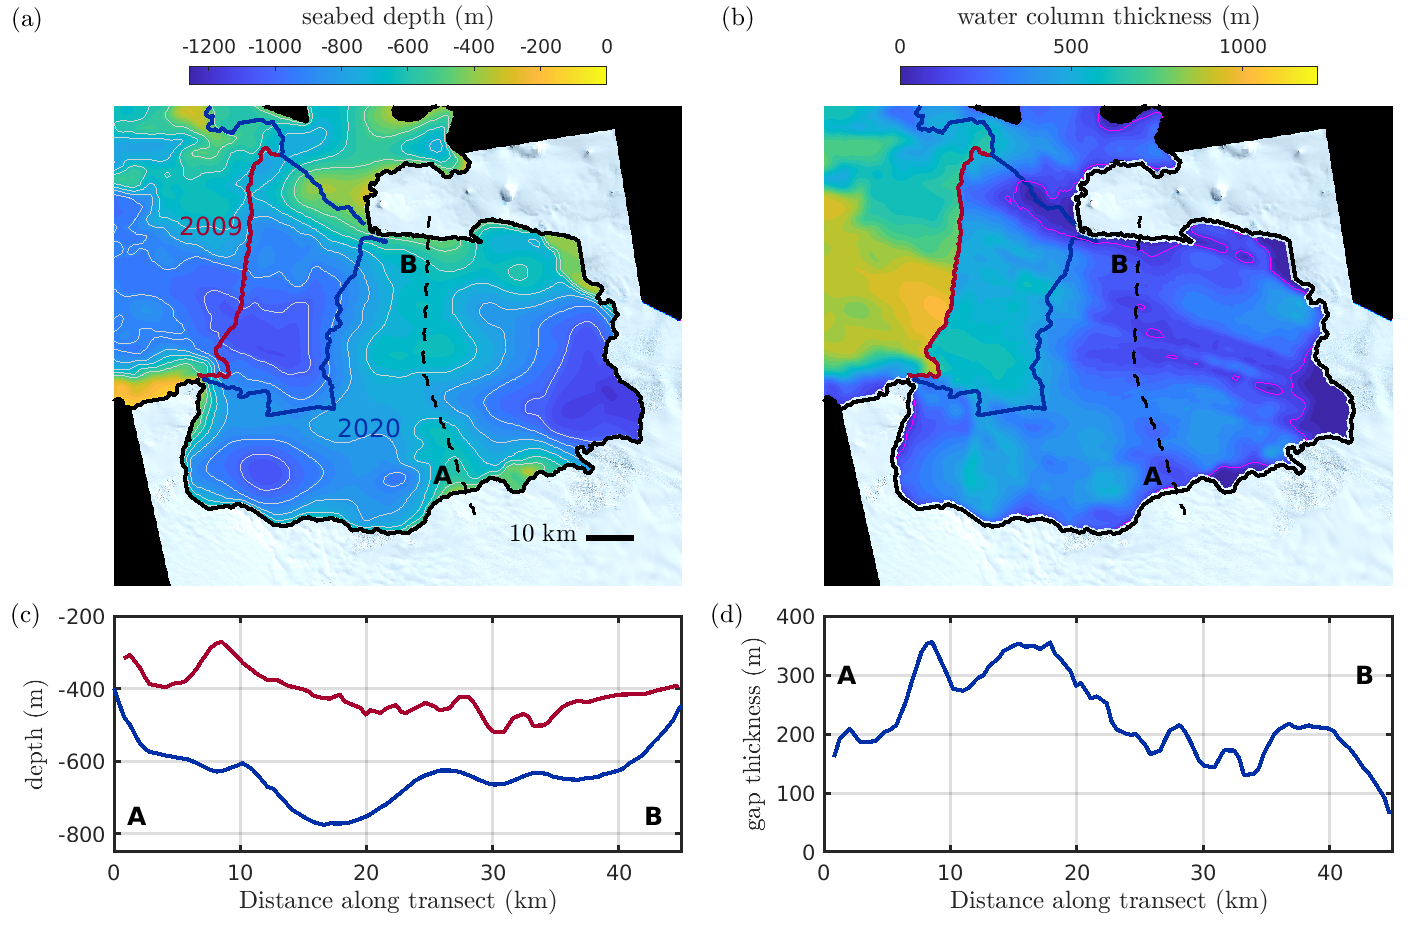
\includegraphics[width = \textwidth]{../make_figures/plots/figure1.png}
    \caption{(a) Seabed depth and (b) water column thickness under Pine Island Ice Shelf and in Pine Island Bay (colors) from~\citeA{Dutrieux2014Science}. Also shown are the locations of the ice front in 2009 (red line) and 2020 (blue line), as indicated in (a).  The solid black line indicates the grounding line from \citeA{Joughin2010GRL}, and the background image is a Sentinel 2 mosaic from November 2020. The black dashed line indicates the approximate location of the crest of the seabed ridge. The magenta contour in (b) corresponds to 125~m  water column thickness. (c) Seabed bathymetry (blue) and ice draft (red) taken along the black dashed line in (a)--(b). (d) Plot of the ridge-seabed gap measured along the black dashed black line in (a) [i.e. the difference between the red and blue lines in (c)]. }
    \label{fig:figure1}
\end{figure}


%ridge in PIG makes pycnocline picture more complicated
However, for PIG specifically, this simple `pycnocline depth' picture is complicated by the presence of a seabed ridge in the ice shelf cavity. This ridge is located several tens of kilometers downstream of the grounding line, and protrudes up to three hundred meters above the neighboring seabed (black dashed line in figure~\ref{fig:figure1}a). In combination with the ice shelf directly above it, the ridge acts as a topographic barrier that restricts the access of CDW to an inner cavity which has formed between the ridge and the grounding line since the ice shelf grounding line retreated from this ridge in a process initiated in the late 1940s~\cite{Jenkins2010NatureGeo, DeRydt2014JGeophysResOceans, DeRydt2016JGeophysResEarthSurf, Smith2017Nature}. This cavity geometry means that the strength of the topographic barrier (i.e. how much its presence affects ice shelf melting) is strongly dependent on the pycnocline depth: at its shallowest, the pycnocline sits above the depth of the ridge crest, and a large amount of modified CDW is able to spill into the inner cavity~\cite{Dutrieux2014Science}; in contrast, at its lowest, the pycnocline sits some way below the ridge crest and CDW access is severely restricted.  The presence of the seabed ridge thus contributes to the strong sensitivity of PIIS melting to hydrographic conditions in Pine Island Bay (PIB): \citeA{Dutrieux2014Science} reported that the total freshwater flux from the fast flowing part of PIG in 2009 (80~km\textsuperscript{3} year\textsuperscript{-1}), when the pycnocline was at its shallowest depth on record~\cite{Webber2017NatureComms}, was more than double its value in 2012 (37~km\textsuperscript{3}~year\textsuperscript{-1}), when the pycnocline was at the second-lowest recorded depth.

%another thing we have seen is significant calving events
In addition to its unique topographic control on melt rates, the recent calving of PIIS also stands out amongst Amundsen Sea terminating ice shelves. Mass loss from the Antarctic ice sheet is dominated by calving and melting~\cite{Rignot2013Science}; in equilibrium, these losses must balance the upstream accumulation of ice. The recent retreat of the ice front of PIIS, however, suggests that the calving rate is far higher than would be required to maintain an equilibrium: the ice front retreated approximately 26 km between 2009 and 2020 (figure~\ref{fig:figure1}a), with the majority of this retreat happening over the period 2015--2020~\cite{Lhermitte2020PNAS, Joughin2021ScienceAdv}. This corresponds to a more-than-doubling of the calving rate, from approximately 4~km~year\textsuperscript{-1} prior to 2015 to approximately 9~km~year\textsuperscript{-1} in the period 2015--2020 [the flow speed at the ice front, for context, is approximately 5~km~year\textsuperscript{-1} \cite{Joughin2021ScienceAdv}].

%at present, the ridge is located approx x km downstream of the ridge crest. The changes some far have been implicated in a speed up because of a loss of buttressing, but might the changes have also led to a relaxation of the topographic barrier and thus and increase in melt rates (that would only be evidenced on longer timescales(?)) [key question one]
As of 2020, the ice front is located approximately 20~km downstream of the ridge (figure~\ref{fig:figure1}a); the ice front is now closer to the ridge crest than it is to the location of the ice front in 2009. The loss of buttressing associated with this retreat of the ice front can explain the acceleration of PIG since 2015~\cite{Joughin2021ScienceAdv}. Given that the topographic barrier to CDW relies on the combination of ice draft \textit{and} seabed ridge, the recent calving events beg the following question: has this calving relaxed the topographic barrier, leading to significant changes in melting on PIIS? Increased melting of ice shelves can lead to further reductions in ice shelf volume and thus buttressing, ultimately leading to ice shelf acceleration, thinning and grounding line retreat.

%but also, in future, we might have further calving events because or preconditioning and or MICI that might bring to ridge to the crest. How might these potential future calving events lead to changes in melt rates? [key question two]
In addition to considering the effect on melt rates of calving events that have already happened, one might also consider how melt rates might respond to possible future calving events. It has been suggested that further significant calving of PIIS is likely: damage to the ice shelf that has already occurred is thought to have preconditioned PIIS to collapse~\cite{Lhermitte2020PNAS}. \blue{Furthermore, there is a theoretical `calving-melting' feedback loop in which calving enhances ice shelf melting, resulting in reduced buttressing and thus ice acceleration, ultimately resulting in ice shelf damage and thus further retreat. Here, we test the first link in this chain of events.} %Jan would like a caveat here, but I think that can wait until the discussion? Could add something like: "other links in this chain have been considered in detail elsewhere (see for example ...), but our study is the first to consider how calving might affect melt rates." This has the added benefit of making explicit the novelty of this paper?}
 \red{Additionally, there is a theoretical feedback loop in which damage leads to calving, resulting in reduced buttressing and thus ice acceleration, which promotes further damage. We expect further calving as part of this feedback process, which also interacts with unbalanced melting.}

In this study, we assess how, and why, melt rates on PIIS might respond to past, and possible future, calving events. To do so, we use a numerical general circulation model to simulate the ocean circulation in both an idealized setup whose geometry captures the salient characteristic features of PIIS and its cavity (most notably, a seabed ridge whose crest is in proximity to the ice shelf base), and a realistic setup, whose geometry closely matches real world conditions for PIIS. We begin in \S\ref{S:Experiment} with a description of the idealized experiments, setting out details of the ocean model used and the experimental setup. We identify one such experiment as a baseline, and present the results of this experiment in \S\ref{S:Baseline}. In \S\ref{S:Results:lc}, we describe how, and why, the melt rate varies as calving proceeds from this baseline. In the following two sections, we discuss how the picture of melt response to calving presented in \S\ref{S:Results:lc} changes when the cavity geometry (\S\ref{S:Results:H}) and far field ocean conditions (\S\ref{S:Results:P}) are altered. In \S\ref{S:Realistic} we describe and present the results of  the realistic experiments. Guided by the results of the idealized experiments, we assess the expected response of melt rates under PIIS to calving events. Finally, we discuss the implications of our results in \S\ref{S:Discussion}, and summarize the key results in \S\ref{S:Summary}.


\section{Experiment Details}\label{S:Experiment}
%broad overview of the experiemnts

\begin{figure}
    \centering
    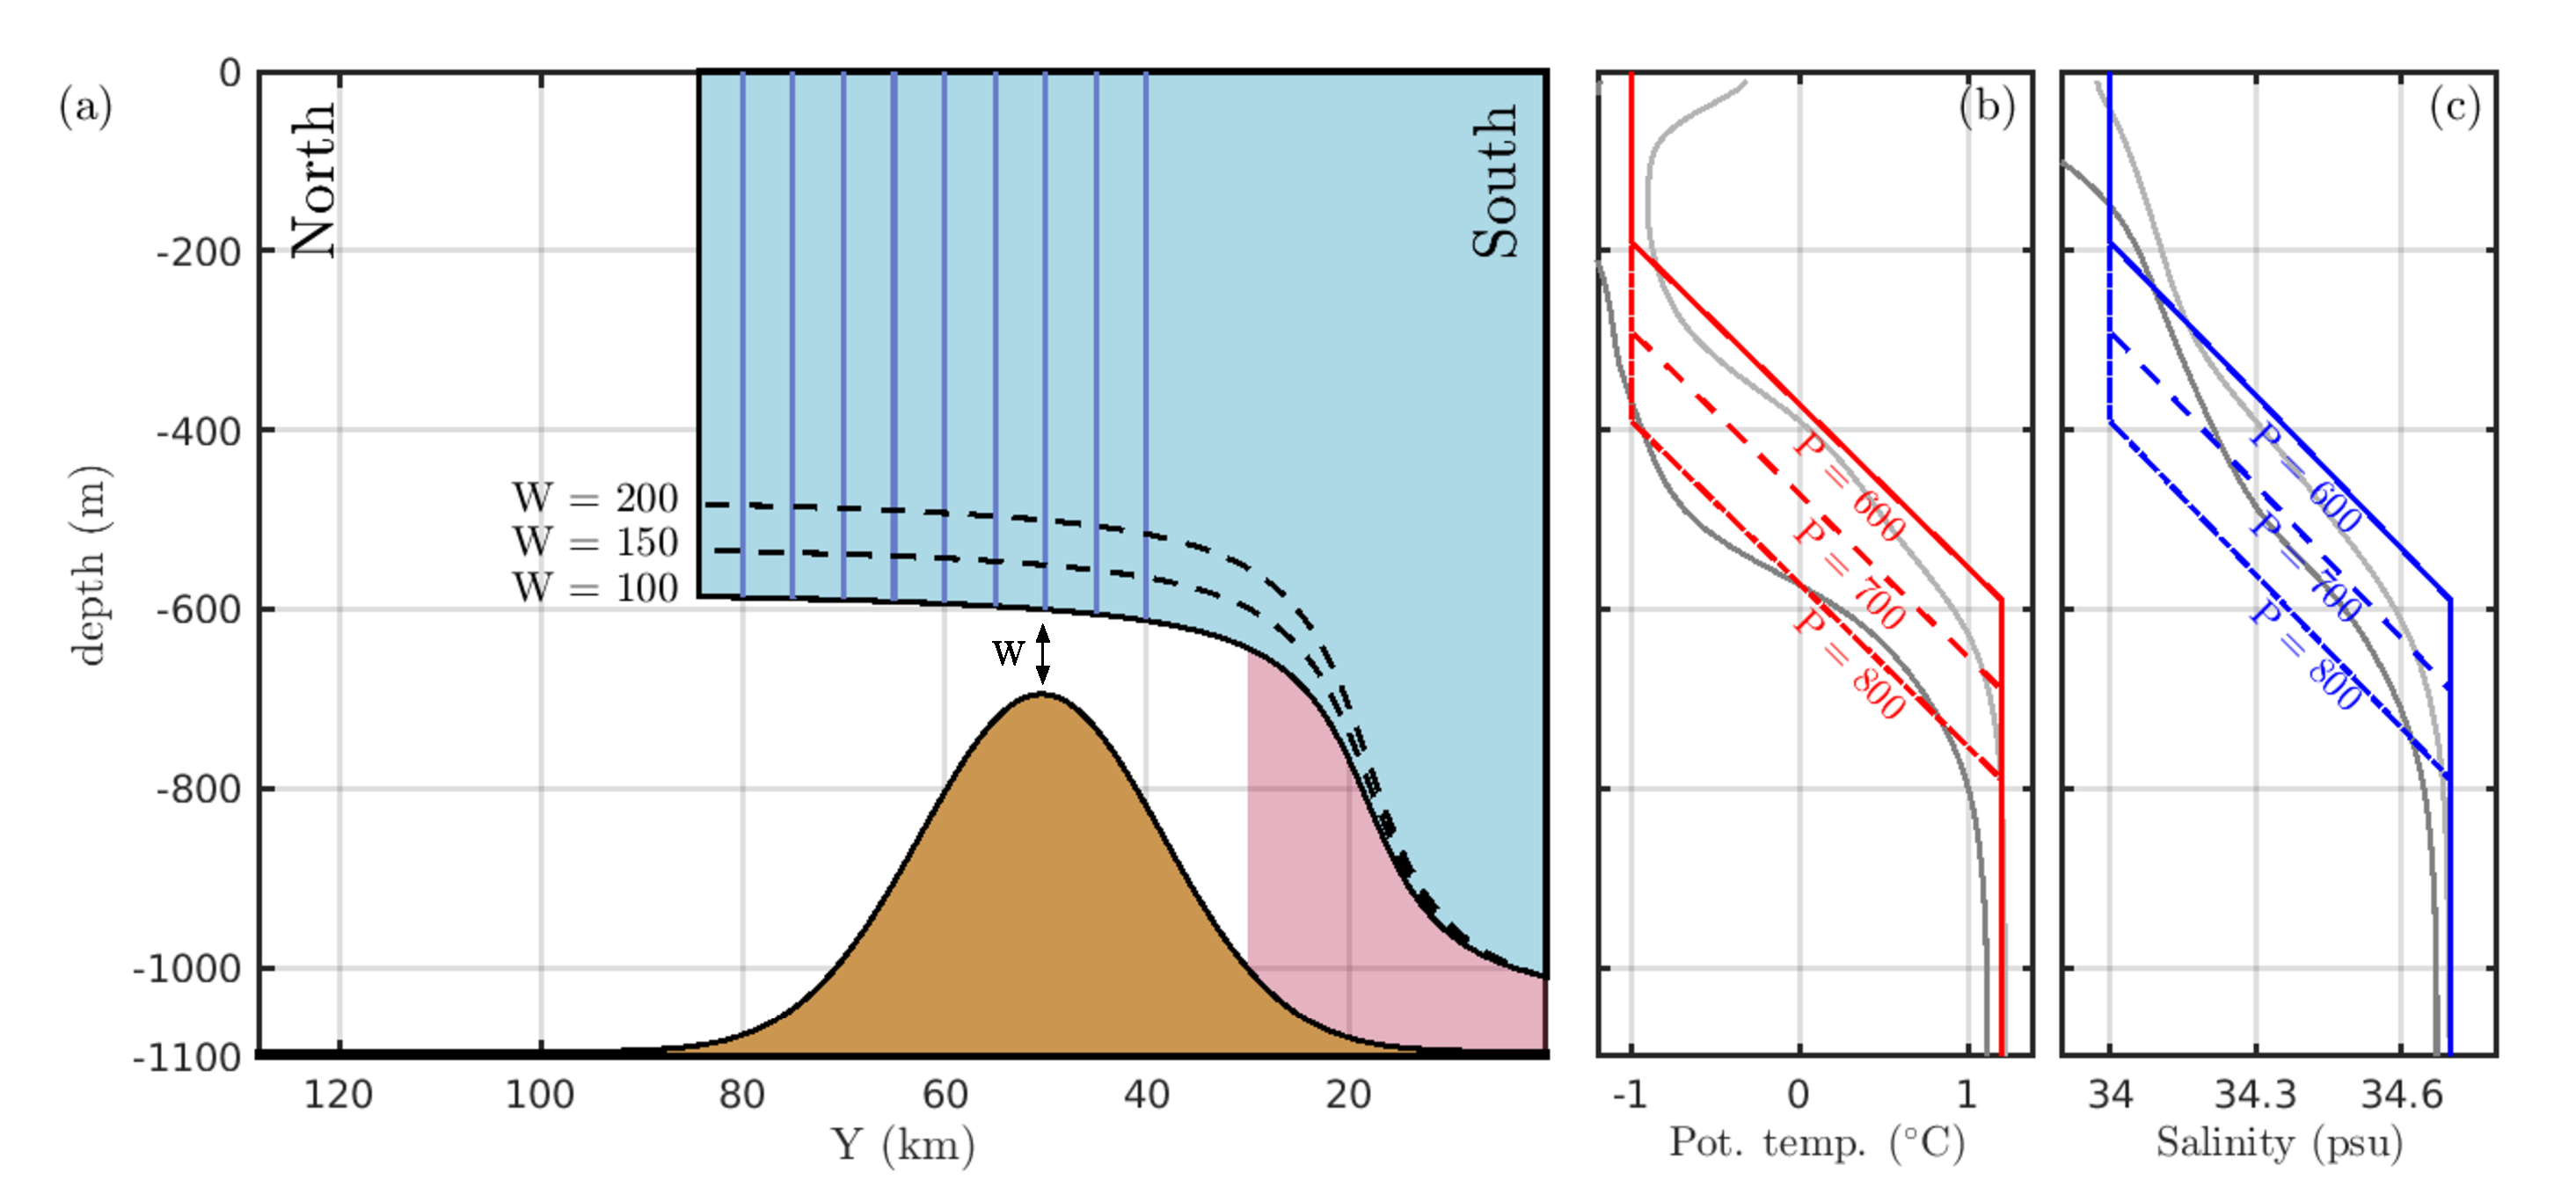
\includegraphics[width = \textwidth]{../make_figures/plots/figure2.pdf}
    \caption{(a) Schematic diagram of the experimental setup. The domain is uniform in the zonal direction (into the page), with extent 48~km. The ocean domain consists of the gridded area, which is bordered by a static ice shelf in $Y < 84$~km (shaded blue) and a seabed (shaded brown), which features a prominent ridge. Solid, dashed and dot-dashed black curves indicate the location of the ice shelf base for $W=100$~m, $W=150$~m, and $W=200$~m, respectively, as labelled (the profile of the ice shelf base is defined in equation~\eqref{E:Experiment:Draft}). Solid blue lines indicate the series of ice front positions considered, which are located at 80, 75, 70, 65, 60, 55, 50, 45, and 40~km offshore of the southern end of the domain at $Y = 0~\text{km}$ (the $Y$-axis is oriented in this way for consistency with the orientation of PIG in practice, see figure~\ref{fig:figure1}). The shaded red region indicates the inner cavity, defined as areas within 30~km of the southern end of the domain. (b) Temperature and (c) salinity profiles used in the experiments. Different line styles correspond to different values of the pycnocline depth parameter $P$ as follows: $P=600$~m (solid), $P=700$~m (dashed), $P=800$~m (dot-dashed). Light and dark gray lines correspond to temperature and salinity profiles taken from conductivity, temperature, and depth measurements in Pine Island Bay during the austral summers of 2009~\cite{Jacobs2011NatureGeosci} and 2012~\cite{Dutrieux2014Science}, respectively.}
    \label{fig:figure2}
\end{figure}

In this section, we describe the experiments performed in an idealized setup, which we refer to as `idealized experiments'. The idealized experiments have essentially the same setup as~\citeA{DeRydt2014JGeophysResOceans}, albeit it with n updated model configuration, and sections of the ice shelf removed to simulate calving. The domain features a seabed ridge and ice shelf (see figure~\ref{fig:figure2}a) which are both uniform in the zonal direction (and thus so too is the ridge-draft gap between them). In practice, however, the ridge-draft gap is non-uniform (figure~\ref{fig:figure1}c--d); to capture the effect of this variation, we consider the melt response to calving for different thicknesses of the ridge-draft gap. We also consider several different far-field ocean conditions (`hydrographic forcings'): as discussed in \S\ref{S:Introduction}, PIIS melt rates have a sensitive dependence on the hydrographic forcing, via the depth of the pycnocline; we therefore postulate that the melt response to calving might similarly have a sensitive dependence on the hydrographic forcing, and investigate this effect. The role of these idealized experiments, with a highly simplified geometry, is to allow us to isolate the important roles that the ridge-draft gap and the hydrographic forcing play in the melt response to calving, as well as elucidate the physical mechanisms responsible for these changes.

We perform a total of 90 idealized experiments, each corresponding to a unique triplet of parameters which describe the ridge-draft gap, the hydrographic forcing, and the position of the ice front. These parameters are described in the following two sections. By systematically shifting the ice front towards the (fixed) grounding line between experiments, we simulate calving (and use that name to describe this procedure), but stress that our model includes neither calving dynamics, nor associated processes such as mélange formation. Within each experiment, we solve for the three-dimensional ocean circulation and associated melt rates simultaneously using the MIT general circulation model (MITgcm)~\cite{Marshall1997JGROceans}. Other than removing sections of the ice shelf, the ice shelf geometry does not change between experiments. Ice shelves themselves enter the ocean model via the exchange of heat and salt at the ice-ocean interface and a steady pressure loading on the ocean surface (i.e. ice-dynamics are not taken into  consideration when determining the cavity geometry); a steady description of ice shelves is sufficient to assess the response of melt rates to ice shelf calving, which occurs on a timescale much shorter than that on which the ice responds dynamically to perturbations in melting. In the following sections, we provide further details of the ocean model and experimental setup, including the motivation for our choices of parameters.


\subsection{Details of Ocean Model}\label{S:Experiment:Model}
The MITgcm is a z-level general circulation model that includes a partial-cell treatment of topography, allowing an accurate description of both the seabed and ice draft. Our model grid consists of 110 layers with a vertical spacing of $\mathrm{d}z = 10$~m, and a horizontal resolution of  $\mathrm{d}x=400$~m. We use the MITgcm in hydrostatic mode with an implicit nonlinear free surface scheme, a third-order direct space-time flux limited advection scheme, and a non-linear equation of state~\cite{Mcdougall2003JAtmosOceanTech}. The Pacanowski-Philander \cite{Pacanowski1981JPhysOcean} scheme parametrizes vertical mixing. Constant values of 15 and 2.5
m\textsuperscript{2} s\textsuperscript{-1} are used for the horizontal Laplacian viscosity and horizontal diffusivity, respectively. The equations are solved on an $f$-plane with $f = -1.4\times10^{-4}~\text{s}^{-1}$.

In each experiment, the simulation is run for twelve months using a timestep of 30~\si{seconds}, after which the configuration is quasi-steady state. (In each simulation, the field of melt rate is everywhere within 95\% of its final value after three months.) All results presented here are averaged over the final two months of the simulations.

As mentioned, ice shelves impact on the ocean state via the exchange of heat and salt at the ice-ocean interface. This exchange is implemented using the so-called "three-equation formulation"~\cite{Holland1999JPhysOcean}, whose implementation in MITgcm has been described in detail elsewhere \cite[for example]{Losch2008JGeophysResOceans, DeRydt2014JGeophysResOceans,Dansereau2014JGROceans} and so we do not describe this implementation in detail. \red{It is useful to note, however, that the temperature difference between ice shelves and the adjacent ocean boundary layer is one to two orders of magnitude smaller than the temperature associated with phase changes ($L/c \approx -84{}^\circ$C, where $L=3.35\times10^5$ is the latent heat of fusion, and $c_p=3947~\si{\joule \kilogram}^{-1}$ is the specific heat capacity of water). Thus, thermal exchange across the ice-ocean interface is typically dominated by latent heat (over heat conduction into the ice). With latent heat dominated thermal exchange, the three equation formulation simplifies to give the melt rate $\dot{m}$ as}
\blue{It is useful to note, however, that thermal exchange across the ice-ocean interface is typically dominated by latent heat [over heat conduction into the ice~\cite{Holland1999JPhysOcean}]; in the case of negligible heat conduction, the three equation formulation for melting reduces to}
\begin{equation}\label{E:MeltRate}
    \dot{m} = \frac{c_p \gamma_T (T - T_b)}{L}.
\end{equation}
Here $T$ is the temperature in the mixed layer adjacent to the ice base, which is considered to have a thickness $\mathrm{d}z$ everywhere. In addition, $T_b$ is the temperature at the ice shelf base, which must be at the local (depth and salinity dependent) freezing point, and $\gamma_T$ is a heat exchange coefficient, which parametrizes exchange across this boundary layer. The heat exchange-coefficient $\gamma_T$ has a weakly non-linear dependence on $u^*$, the ocean speed in the boundary layer adjacent to the ice shelf base~\cite{Holland1999JPhysOcean}. If this relationship were perfectly linear, $\gamma_T \propto u^*$, equation~\eqref{E:MeltRate} would yield
\begin{equation}\label{E:MeltRateUdT}
    \dot{m} \propto u^* (T - T_b).
\end{equation}
We shall return to equation~\eqref{E:MeltRateUdT} when diagnosing the mechanisms responsible for the melt rate response to ice shelf calving.

With the exception of the drag coefficient at the ice shelf base, we use parameter values from \citeA{Holland1999JPhysOcean} in the three equation formulation. The drag coefficient in the three equation formulation of melting is set to $4.5\times10^{-3}$, a value that is more appropriate for Pine Island Glacier (see \S\ref{S:Realistic}). (Note that the drag coefficient that enters the momentum balance, which can be set independently, remains at the standard value of $2.5\times 10^{-3}$.)


\subsection{Ice Shelf Geometry and Seabed Bathymetry}\label{S:Experiment:Geometry}
The geometry of the idealized setup is shown schematically in figure~\ref{fig:figure2}a. It is uniform in the zonal direction, along which the $X$-axis is aligned, and the $Y$-axis is aligned along the meridional direction. Note that although PIG is aligned approximately east-west, we orient this idealized model north-south, as is standard~\cite{Grosfeld1997JGROceans, DeRydt2014JGeophysResOceans} and results are independent of this choice of orientation.

The seabed has a shifted Gaussian profile,
\begin{equation}\label{E:Experiment:Bed}
    b(X,Y) = -1100 + 400 \exp\left[-\frac{\left(Y - 50\times 10^3\right)^2}{2\sigma^2}\right],
\end{equation}
where $\sigma = 12$~km is the length scale over which this profile decays towards zero. The profile~\eqref{E:Experiment:Bed} corresponds to a ridge that peaks at a height of 400~m above the surrounding bathymetry. This peak occurs 50 km from the southern end of the domain at $Y=0$~km, which we consider to be the grounding line (figure~\ref{fig:figure2}a).

In reality, the variability in both PIIS draft and the height of the seabed ridge result in a ridge-draft gap that varies between approximately 100 m at its thinnest, to greater than 300 m at its thickest (figure~\ref{fig:figure1}c--d). Since we use the same, zonally uniform, seabed geometry (and, in particular, the same ridge height) in all of our idealized experiments, we aim to gain insight into the effect of variation in the ridge-draft gap by considering several different values of $W$ -- the vertical distance between the crest of the seabed ridge and the ice shelf base (figure~\ref{fig:figure2}a). In our setup, $W$ enters the model only via the ice profile; following~\citeA{DeRydt2014JGeophysResOceans}, we use an ice shelf draft that is given by
\begin{equation}\label{E:Experiment:Draft}
    H(Y) = \begin{cases}
    \left(\frac{310 + W}{2.64}\right)\tan^{-1}\left(\frac{Y}{5882} -3\right) & \text{for}~Y < Y_f,\\
    0  & \text{for}~Y \geq Y_f.
    \end{cases}
\end{equation}
Here $Y_f$ is the variable location of the ice front (see below). We stress that the ice draft profile~\eqref{E:Experiment:Draft} is not obtained from ice dynamics considerations, but selected for its qualitative similarity to PIIS: it includes a flatter section offshore of the ridge and a steeper section inshore of the ridge, thus resembling variations in the basal slope that have been inferred from radar and satellite data. Note that the combination of the bathymetry~\eqref{E:Experiment:Bed} and ice shelf draft~\eqref{E:Experiment:Draft} means that the water column thickness is small, but nonzero at the grounding line (figure~\ref{fig:figure2}); this is because the MITgcm requires at least two grid cells in the vertical direction to permit horizontal transfer.

We consider three different values of $W$ here: $W=100$~m, $W=150$~m, and $W=200$~m. The smallest value, $W=100$~m, corresponds to the minimum observed ridge-draft gap under PIIS (figure~\ref{fig:figure1}b, c), while the largest value, $W=200$~m, corresponds to an upper bound, above which there is little melt response to calving, as we shall see.

As mentioned, the front position $Y_f$ is systematically reduced between experiments to simulate calving. We consider a total of ten different ice front positions, using $Y_f=84$, $80$, $75$, $70$, $65$, $60$, $55$, $50$, $45$, and $40~\text{km}$, which correspond to calved lengths of $l_c=0$, $4$, $9$, $14$, $19$, $24$, $29$, $34$, $39$, and $44~\text{km}$, respectively. Those experiments with $l_c = 0~\text{km}$ are referred to as `uncalved' experiments, serving as a benchmark against which results for $l_c >0~\text{km}$ are compared. There are both pragmatic and physical reasons for choosing this particular range of values for $l_c$: the setup with $\ell_c = 0$~km has an ice shelf whose length roughly agrees with the observed distance of the ice front from the PIG grounding line in 2009, before significant calving took place in the late 2010s; the largest value, $l_c = 44~\text{km}$, is chosen as a compromise between allowing us to consider scenarios in which the ice front has been retreated significantly beyond the ridge, whilst retaining a large area that is shared by each experiment (as we discuss further in \S\ref{S:Baseline}, the area over which melt rates are averaged must be invariant to calving for a robust assessment of the melt response to calving).


\subsection{Hydrographic Forcing}\label{S:Experiment:Hydrography}
For each unique value of $W$ and $l_c$, we perform three experiments, each with a different hydrographic forcing. Comparing the results of these experiments gives us an indication of the sensitivity of our results to hydrographic forcing. The range of these hydrographic forcings covers that which is observed in practice (see below).

The hydrographic forcing is imposed on the model by means of a restoring boundary condition at the northern end of the domain ($Y = 128$~km, figure~\ref{fig:figure2}a): at this boundary, the temperature and salinity are restored to specified vertical profiles, shown in figure~\ref{fig:figure2}b and c, respectively, over a distance of five horizontal grid cells (total length 2 km) with a restoring timescale that varies from 12~hours at the boundary to 60~hours in the interior. (We apply a free slip boundary condition at the southern, western, and eastern sides of the domain.) The specified temperature and salinity profiles are piecewise linear functions of depth: they are constant in both an upper (temperature $-1^\circ$C, salinity $34$~PSU) and lower layer (temperature $1.2^\circ$C, salinity $34.7$~PSU), and these layers are separated by a pycnocline of 400~m thickness, across which the temperature and salinity vary linearly. The pycnocline begins at a variable depth $P$ (a higher $P$ corresponds to a deeper pycnocline), which parametrizes the whole profile (figure~\ref{fig:figure2}b, c); the three hydrographic forcings we consider have $P=600$ m, 700 m, and 800 m.

%why do we choose these conditions
These piecewise linear profiles are approximations to typical conditions for Pine Island Bay~\cite{Jacobs1996GRL, Dutrieux2014Science, Jenkins2018NatureGeo} (see figure~\ref{fig:figure2}b--c). As mentioned, the record of hydrographic conditions in Pine Island Bay (PIB) has revealed significant variability in the depth of the pycnocline on interannual timescales~\cite{Dutrieux2014Science}; the profiles with $P=600$~m and $P=800$~m are approximations to profiles observed in PIB in the years 2009 and 2012, respectively (figure~\ref{fig:figure2}b, c). These two years approximately span the range of observed conditions: in 2009, the average depth of the pycnocline was at its shallowest level on record~\cite{Webber2017NatureComms}, while in 2012 the average depth of the pycnocline was at its second-deepest level on record.

%wrap up the experiments:\
In summary, we perform a total 90 idealized experiments. Each is uniquely identified by a $(W,~P,~l_c)$ triplet, where $W$ $\in \{100,~150,~200\}~\text{m}$, $P$ $\in \{600, 700, 800\}~\text{m}$, and $l_c \in \left\{0,~4,~9,~14,~19,~24,~29,~34,~39,~44\right\}~\text{km}$. We consider the experiment with $W=100$~m, $P=600$~m, and $l_c=0$~km to be the baseline; this corresponds to the extreme scenario with the narrowest ridge-draft gap (the strongest topographic barrier), the hydrographic forcing with the shallowest pycnocline (thickest CDW layer), and an uncalved ice shelf. In the following section, we describe the results of the baseline experiment. In \S\ref{S:Results:lc}, we describe the results of applying the calving perturbation to the baseline, presenting results of those experiments with  $W=100~\text{m},~P=600~\text{m},~l_c>0~\text{km}$; i.e. we describe the melt response to calving for $W=100~\text{m}$, $P = 600~\text{m}$. In \S\ref{S:Results:H} and~\ref{S:Results:P}, we respectively describe how this picture of melt response to calving changes for the different values of $W$ and $P$ considered.


\section{Results for the Baseline Experiment ($W$=100~m, $P$=600~m)}\label{S:Baseline}
In this section, we describe the results for the baseline experiment with $W=100~\text{m}$, $P=600~\text{m}$, and $l_c=0~\text{km}$. This configuration corresponds to the solid lines in figure~\ref{fig:figure2}.

\begin{figure}
    \centering
    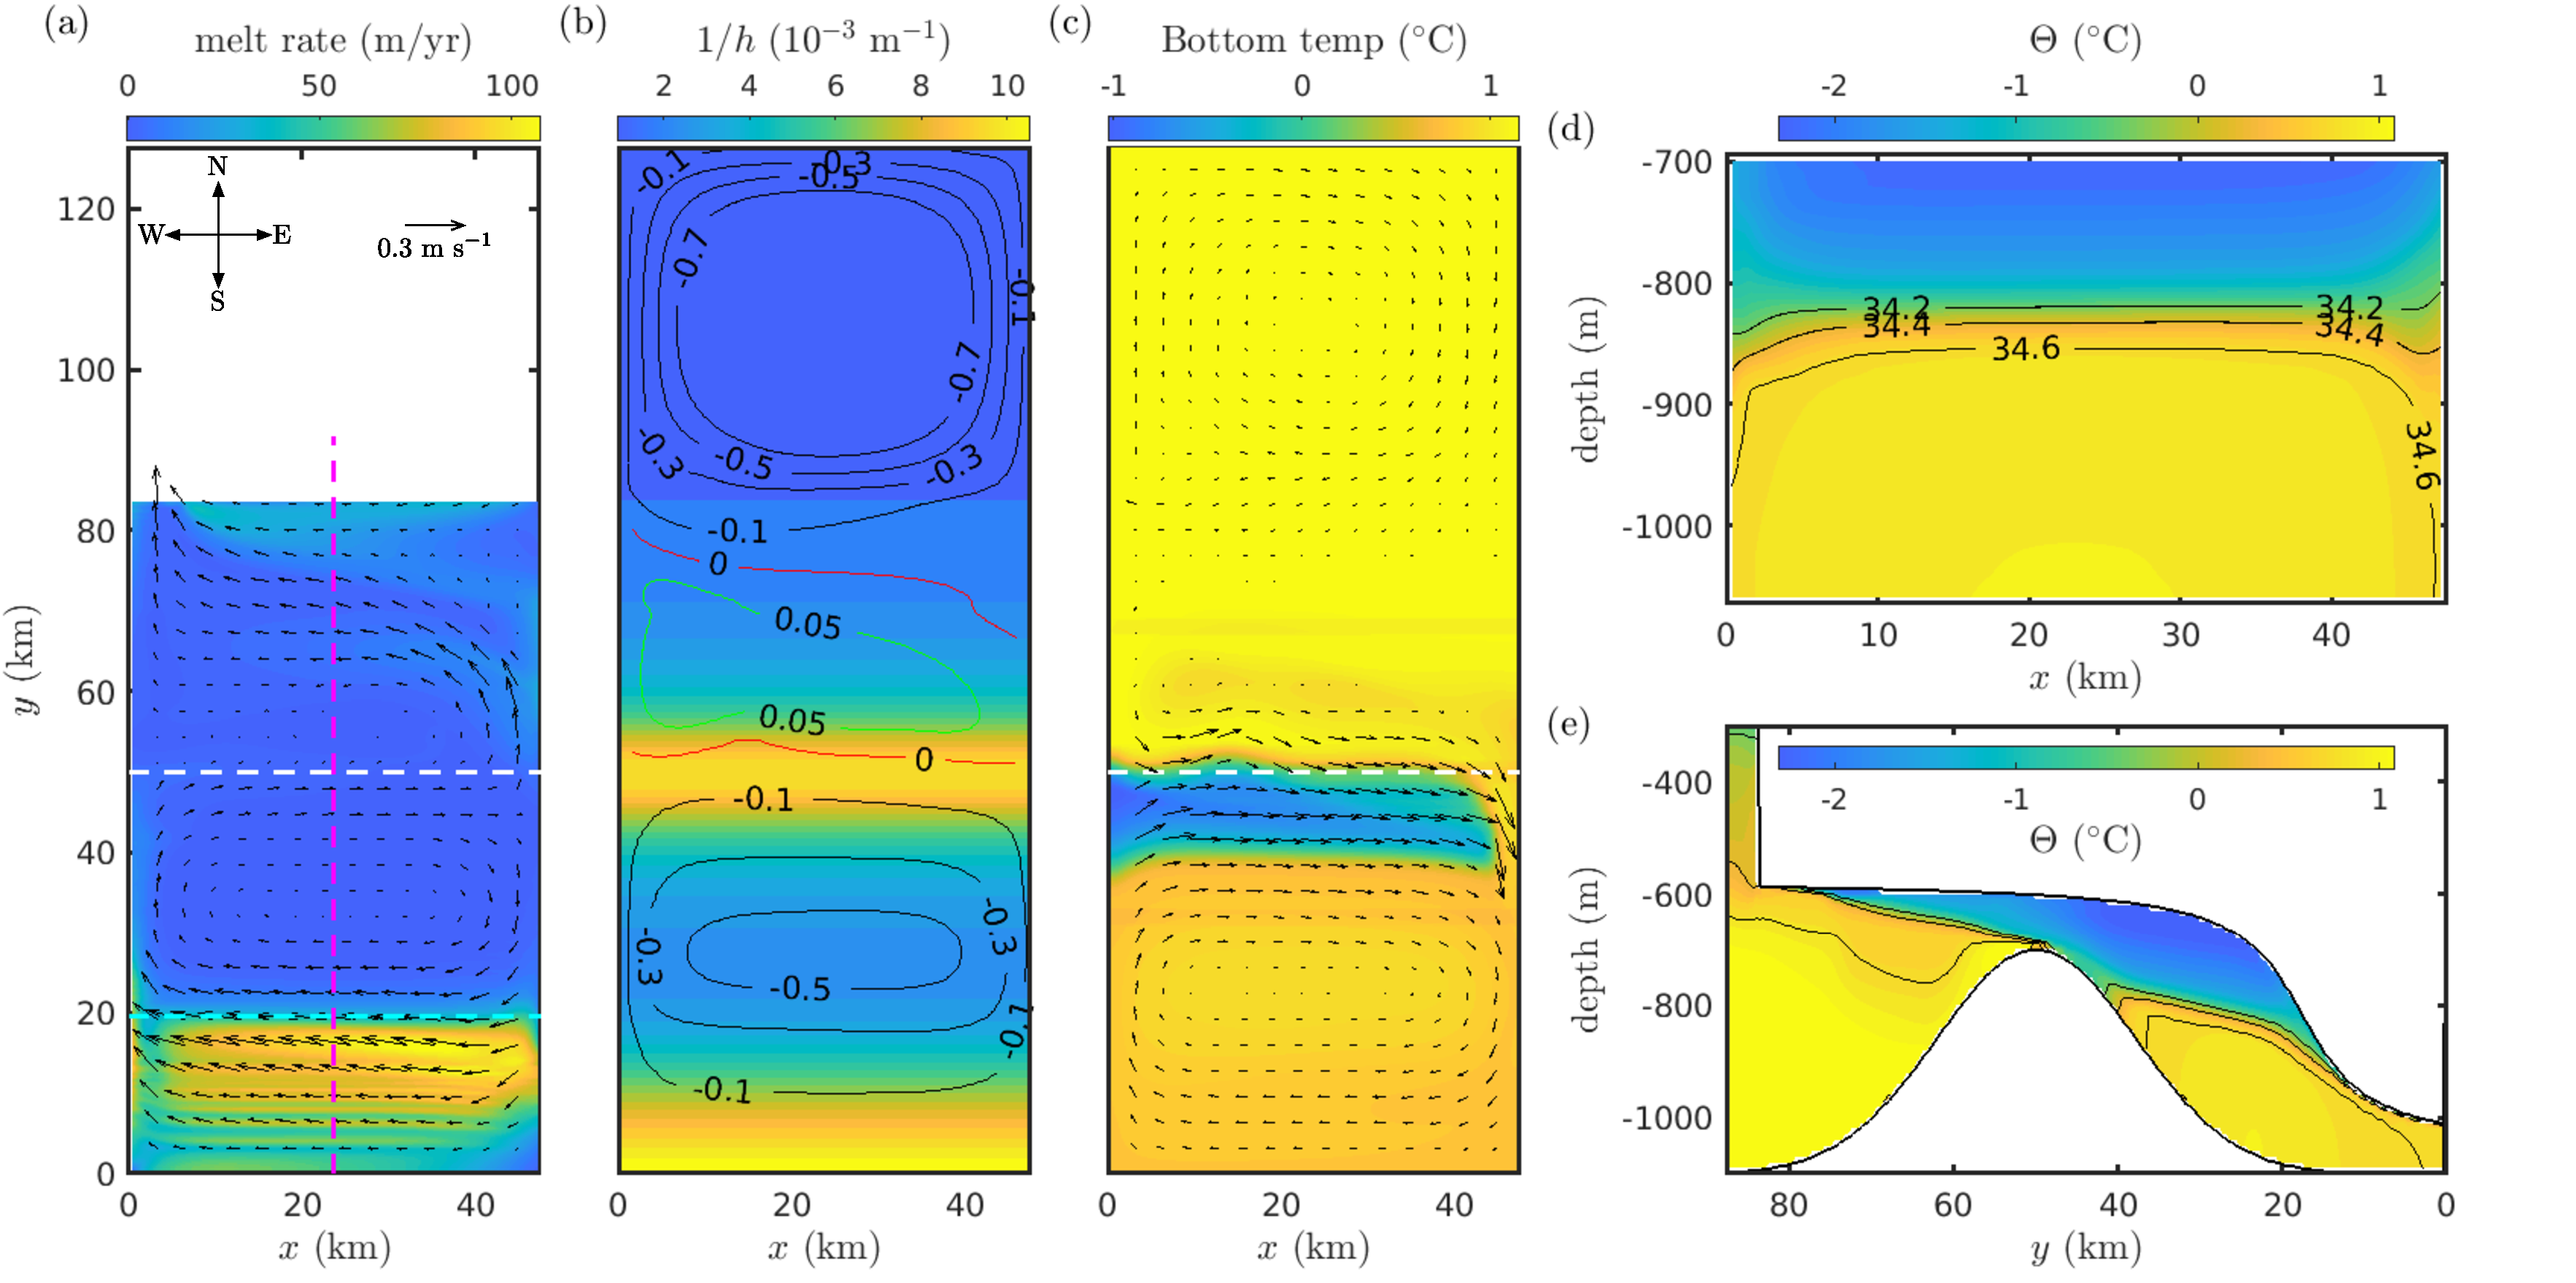
\includegraphics[width = \textwidth]{../make_figures/plots/figure3.pdf}
    \caption{Ice-ocean properties that characterize the baseline experiment, with $W = 100$~m, $P = 600$~m, and $\ell_c = 0$~km. (a) Melt rate (colors) and ice-ocean boundary layer velocities (arrows, every fifth velocity vector is plotted), averaged over the three grid cells adjacent to the ice-ocean interface. White areas correspond to open ocean. The white dashed line indicates the location of the ridge crest, the cyan dashed line indicates $y=20~\text{km}$ [along which the section in (d) is taken], and the magenta dashed line indicates the center line $x = 24~\text{km}$ [along which the section in (e) is taken]. (b) Inverse water column thickness $1/h$ (colors) and barotropic stream function (contours, in units of Sv) at levels 0.05 (green) 0 (red), -0.1, -0.3, -0.5, and -0.7~Sv (all black). (c) Bottom temperature (colors) and bottom current (arrows) averaged over the three grid cells closest to the seabed. The scale bar for velocity vectors in (a) is also appropriate for (c). (d) Zonal cross-section taken at $y=20~\text{km}$ up to the ice shelf base, showing potential temperature (colors) and salinity contours at the 34.2, 34.4, and 34.6~PSU levels, as indicated. (e) Meridional cross-section of temperature and salinity (with colors and contours as in (d)), taken along the centerline $x = 24$~km.}
    \label{fig:figure3}
\end{figure}

%describe each of what we see: melt rate, general observations
Ice-ocean properties that characterize the baseline simulation are shown in figure~\ref{fig:figure3}. Melt rates (figure~\ref{fig:figure3}a) are below  20~m~year\textsuperscript{-1} everywhere, except for a region located within 20~km of the grounding line, where melt rates reach a maximum of approximately 120~m~year\textsuperscript{-1}. The average melt rate over the whole shelf is approximately 20~m~year\textsuperscript{-1}; this is lower than the value of 33$\pm$2~m~year\textsuperscript{-1} that was estimated by~\citeA{Jenkins2010NatureGeo} based on observations in Pine Island Bay in 2009, to which the $P=600$~m case corresponds (figure~\ref{fig:figure2}b, c). This discrepancy is in the expected direction: the baseline simulation corresponds to the extreme scenario in which the ridge-draft gap is set everywhere to the minimum gap that is observed in practice, impeding the supply of warm water across the ridge.

%introduce the idea of the inner cavity, why do we use this metric
At this point, we introduce the definition on the `inner cavity' as the area of the ocean domain that is located within 30~km of the southern boundary, indicated by the red-shaded region in figure~\ref{fig:figure2}a). We use the mean melt rate in the inner cavity, referred to henceforth as the `inner cavity melt rate', as a single metric to quantify changes in melt rate with calving. Since the melt rate is highly spatially variable (figure~\ref{fig:figure3}a) it is necessary to consider a fixed area that is common to each simulation, when assessing changes in melt rate with calving. Indeed, averaging over the whole shelf, for example, would make smaller shelves appear to have anomalously large melt rates, since the region of high melt close to the grounding line would occupy a greater proportion of the entire shelf. Our choice of 30~km in the definition of the inner cavity region reflects a compromise between enabling simulations in which the ice front has calved a significant distance beyond the ridge to be included (the smallest shelf we consider must be larger than the inner cavity region if the entirety of this region is to be included in each simulation), and considering a reasonably large section of the uncalved ice shelf over which the mean melt rate is computed. Crucially, this choice includes the region adjacent to the grounding line, where changes in melt rate are especially important for the dynamics of the grounded ice sheet \cite{Seroussi2014Cryo, Athern2017GRL}. Although the values of inner cavity melt rate \textit{are} dependent on the length chosen in the definition of the inner cavity, we verified that the trends and key results presented here are independent of this choice. The inner cavity melt rate in the baseline simulation is 46~m~year\textsuperscript{-1} (see $l_c = 0$~km in figure~\ref{fig:figure4}a).

%why does the melt rate look like it does
Melt rates are proportional to the product of the ice-ocean mixed layer circulation and thermal driving [see equation~\eqref{E:MeltRateUdT}]. Cavity circulation (figure~\ref{fig:figure3}a, c) is characterized by a geostrophic cyclonic circulation. This circulation is directed northward at the western boundary ($x=0$~km) and southward at the eastern boundary ($x=48$~km). In the inner cavity, the circulation is vigorous to the south of $y=30~\text{km}$, but high melt rates are restricted to south of $y=20~\text{km}$: to the north of $y=20~\text{km}$, a cold and fresh meltwater plume sits adjacent to the ice-ocean interface (figure~\ref{fig:figure3}e) and the thermal driving is therefore much smaller than to the south of $y=20~\text{km}$, where the ice is adjacent to warm water.


%we can use the bsf
\red{When the ice shelf is calved in the subsequent simulations, we change both the buoyancy flux (the total volume of meltwater changes), as well as the water column thickness in those regions of the domain in which the ice shelf is removed.}
\blue{When the ice shelf is calved in the subsequent simulations, the configuration changes in key ways: we change the imposed water column thickness in those regions of the domain in which the ice shelf is removed, and the buoyancy flux that emerges from the simulation is altered (the total volume of meltwater changes).}
 Changes in the water column thickness influence the flow through barotropic dynamics; it is therefore instructive to consider the \red{barotropic stream function for the uncalved simulation first (figure~\ref{fig:figure3}b), and then assess how it changes with calving.}  \blue{barotropic dynamics first for the uncalved simulation, and then assess how they change with calving. As we shall see, the melt response to calving can be accurately diagnosed in terms of barotropic dynamics, and it is therefore sufficient to consider only barotropic dynamics.}
 
\blue{ In the absence of surface and bottom stresses, barotropic velocities $u$ and $v$ must satisfy (see~\cite{Patmore2019JPO}, for example)
 \begin{equation}\label{E:BPVeq}
\frac{\mathrm{D}}{\mathrm{D}t}\left( \frac{f + \zeta}{h}\right) = \frac{\nu}{H}\nabla^2 \zeta,
 \end{equation}
where $h$ is the water column thickness, $\zeta = \partial v / \partial x - \partial u / \partial y$ the relative vorticity,  and $\nu$ the kinematic viscosity. Equation~\eqref{E:BPVeq} implies that potential vorticity (PV),  calculated as $(f + \zeta)/h$ is conserved following the flow, except in regions where viscous stresses are important. Note that if the flow is steady, because the domain is uniform in $x$, equation~\eqref{E:BPVeq} reduces to
\begin{equation}
    v f  \frac{\mathrm{d}}{\mathrm{d}x} \left(\frac{1}{h}\right) + \mathbf{u}.\nabla \left(\frac{\zeta}{h}\right) = \frac{\nu}{H}\nabla^2 \zeta.
\end{equation}
Equation~\eqref{E:BPVeq} implies that in regions where viscous stresses are important, flow generally aligns with contours of constant $f/h$, unless relative vorticity changes. In our idealized domain, contours of constant water column thickness correspond to lines of constant $y$, aligned east-west (figure~\ref{fig:figure3}c). The ice front and the seabed ridge are the two main discontinuities in the water column thickness, and therefore act as PV barriers; these PV barriers divide the domain up into three regions of closed $f/h$ contours: inshore of the ridge, offshore of the ridge (but under the ice shelf), and the open ocean.}

%how can we see where these terms are important
\blue{We can determine which terms in equation~\eqref{E:BPVeq} are important in certain regions of our domain by considering $1/h$, $(f + \zeta)/h$, and the barotropic stream function. We see that barotropic flow predominantly follows contours of constant $f/h$ (figure~\ref{fig:figure3}c), aligned east-west. Contours of constant $(f + \zeta)/h$ deviate from these east-west aligned contours at the domain boundaries, indicating where relative vorticity plays an important role in the barotropic flow. There are two main regions where streamlines of the barotropic flow (contours of constant barotropic streamfunction) deviate from $(f + \zeta)/h$: at the ice front, and at the eastern boundary. In these locations, viscous stresses play an important role, i.e. at the ice front (where vorticity is induced by lateral shear in the water column) and at the eastern boundary (where vorticity is induced by flow that is directed along the ridge, figure~\ref{fig:figure3}b meets the solid boundary), vorticity permits the flow to break the topographic constraint. Importantly, however, the topographic constraint is sufficiently strong along the rest of the ridge that zero barotropic flow is able to cross it.  }

\blue{The eastern boundary current provides the inner cavity with water from offshore of the ridge (figure~\ref{fig:figure3}b). However, the total flux provided by this flow (approximately 0.03~Sv) is small in comparison with the typical barotropic fluxes in the cavity, which are on the order of 0.3~Sv  (figure~\ref{fig:figure3}c). As discussed, the topographic constraint provided by seabed ridge and ice shelf draft prevents barotropic flow across the ridge; in the absence of significant flow across it, the inshore side of the ridge hosts meltwater, which is recirculated rather than flushed out. Water entering at the eastern boundary mixes with this meltwater as it crosses the ridge; although warm water that enters the inner cavity is lightly modified by this mixing, resulting in a bottom temperature that is slightly cooler (approximately 0.8${}^\circ$C) inshore of the ridge than offshore (approximately 1.3${}^\circ$C, see figure~\ref{fig:figure3}b,~e), the intrusion still provides significant heat to the inner cavity for melting.  The ridge crest topographic barrier means that barotropic flow is also constrained within the cavity, resulting in a strongly topographically controlled cyclonic circulation inshore of the ridge, driven by buoyant meltwater flow. }



 \red{Assuming that turbulent and viscous diffusion are negligible, barotropic flow conserves potential vorticity (PV),  calculated as $(f + \zeta)/h$, where $h$ is the water column thickness and $\zeta = \partial v / \partial x - \partial u / \partial y$ the relative vorticity, with $u$ and $v$ the depth-averaged velocity components in the $x$ and $y$ directions, respectively. Conservation of PV means that flow generally aligns with $f/h$ contours, unless relative vorticity changes. In our idealized domain, contours of constant water column thickness correspond to lines of constant $y$, aligned east-west (figure~\ref{fig:figure3}b). The ice front and the seabed ridge are the two main discontinuities in the water column thickness, and therefore act as PV barriers; these PV barriers divide the domain up into three regions of closed $f/h$ contours: inshore of the ridge, offshore of the ridge (but under the ice shelf), and the open ocean.}
 
 
% Maybe just say at the outset that barotropic dynamics are sufficient to explain behaviour (as we shall see), so we'll just focus on those.  Broadly, barotropic flow predominately follows contours of constant 1/h, except at boundaries and ice front. We can see where relative voricity become important by looking at deviations of (f  + zeta)/h from lines of constant 1/h, i.e. looking at where figure 3d is not constant in y: so relative vorticity is important predominately at boundaries. Where the barotropic flow deviates from (f + zeta)/H indicates where viscosity is important, i.e. predomiantely at the ice front and at the eastern boundary. First point: ice front induced viscosity (through shear) allows barotropic flow to break the PV barrier (which will be important in the following section). Second point is important because southward boundary current provides heat for melting (but not much -- small flux across the ridge) (setup , becuas this flux will change in the following). However, this is the only place where flow across the ridge occurs -> PV barrier is strong enough that no flow across ridge. In absecene of significant flow across ridge, meltwater hosted on ridge is recirculated. Water entering mixes.

%Assuming steady, PV contraint term reads f u d/dy(1/h), other two terms are prop. to flow speed. So strong topographic barrier requires high flow speed to balance. 

\red{Regions of closed $f/h$ space promote gyre formation. Offshore of the ridge, a weak anti-cyclonic circulation spins up. Meltwater that crosses the ridge into this region northward from the inner cavity experiences an increase in water column thickness (reduction in $1/h$); in order to maintain a constant PV, water columns must gain relative vorticity, diverting the flow in an anti-clockwise direction (increasing $\partial v / \partial x$ and/or reducing $\partial u / \partial y$). Similarly, as the flow approaches the ridge along the seabed on the western side (increasing $1/h$), it is diverted eastward (figure~\ref{fig:figure3}c). Ultimately, however, the PV barrier in this `narrow gap' ($W=100~\text{m}$) case is sufficiently strong that little flow is able to pass through it (note the zero barotropic contour at the top of the ridge in figure~\ref{fig:figure3}b). Similarly, the ridge crest PV barrier means that barotropic flow is also constrained within the cavity, resulting in a strongly topographically controlled cyclonic circulation inshore of the ridge. Equivalently, the large PV that is generated by glacial melt in the inner cavity is confined within this region.}

\red{There are two main deviations from this barotropic picture: a strong southward boundary current that is set up at the eastern wall of the domain (figure~\ref{fig:figure3}b, c), and a zero depth-mean (baroclinic), vertically sheared overturning circulation, which is driven by glacial melt. Although this overturning circulation flushes the inner cavity with water from offshore of the ridge, it does so far more weakly than even a moderate barotropic flow would be able to accomplish (the total flux across the ridge, into the cavity, is 0.03~Sv, which is small in comparison with the typical barotropic fluxes in the cavity, figure~\ref{fig:figure3}b). As discussed, the PV barrier provided by seabed ridge and ice shelf draft prevents barotropic flow across the ridge; in the absence of significant flow across it, the inshore side of the ridge hosts meltwater, which is recirculated rather than flushed out. Water entering at the eastern boundary mixes with this meltwater as it crosses the ridge; although warm water that enters the inner cavity is lightly modified by this mixing, resulting in a bottom temperature that is slightly cooler (approximately 0.8${}^\circ$C) inshore of the ridge than offshore (approximately 1.3${}^\circ$C, see figure~\ref{fig:figure3}c,~e), the intrusion still provides significant heat to the inner cavity for melting.}

In summary, in the baseline simulation, which has a strong barrier restricting CDW access to the inner cavity, a topographically constrained cyclonic circulation is spun up inshore of the ridge. The large PV that is generated in the inner cavity is confined to that region. A modest current at the eastern boundary provides the inner cavity with lightly modified warm water, which provides a significant source of heat for melting. However, the hosting of cold meltwater on the inshore of the ridge means that melting high melt rates are restricted to a region just downstream of the grounding line.

%We note that despite this simulation corresponding to a topographic barrier that is expected to be stronger than reality, several features are in agreement with observations such as the presence of warm water on the inner cavity, the presence of a strong meltwater plume that is coldest inshore of the ridge, and a weak hydrographic front that forms on the Northern slope of the ridge~\cite{Jenkins2010NatureGeo}.

%figure 4: plots of (a) melt rate and velocity vectors, (b) geostrophic contours and BSF overlain and (c) bottom current and temperature (i.e. a la Jan 2014 paper)
\section{Melt Response to Calving}\label{S:Results:lc}
In this section, we describe how, and why, the inner cavity melt rate responds when the ice shelf in the baseline experiment is calved. The inner cavity melt rate as a function of the calved length $l_c$ is shown in figure~\ref{fig:figure4}a. We see that, while the ice shelf front is located far offshore of the ridge ($l_c< 14$~km), removing sections of ice results in only a weak increase in the inner cavity melt rate. However, as the ice shelf front is retreated further towards the ridge, the melt rate increases dramatically, reaching a maximum of 73~m~year\textsuperscript{-1} (70\% larger than in the uncalved run) when the ice shelf is located approximately 5~km north of the ridge crest. Perhaps surprisingly, retreating the ice front slightly further to sit directly above the ridge crest results in a significant decrease in the inner cavity melt rate of approximately 15\% (from 73~m~year\textsuperscript{-1} to 64~m~year\textsuperscript{-1}). Finally, the inner cavity melt rate is approximately independent of ice front position when the ice front is located onshore of the ridge ($l_c>34$~km).

%figure 5: (a) plot of mean melt rate as a function of extent and (b) millgate decomposition
\begin{figure}
    \centering
    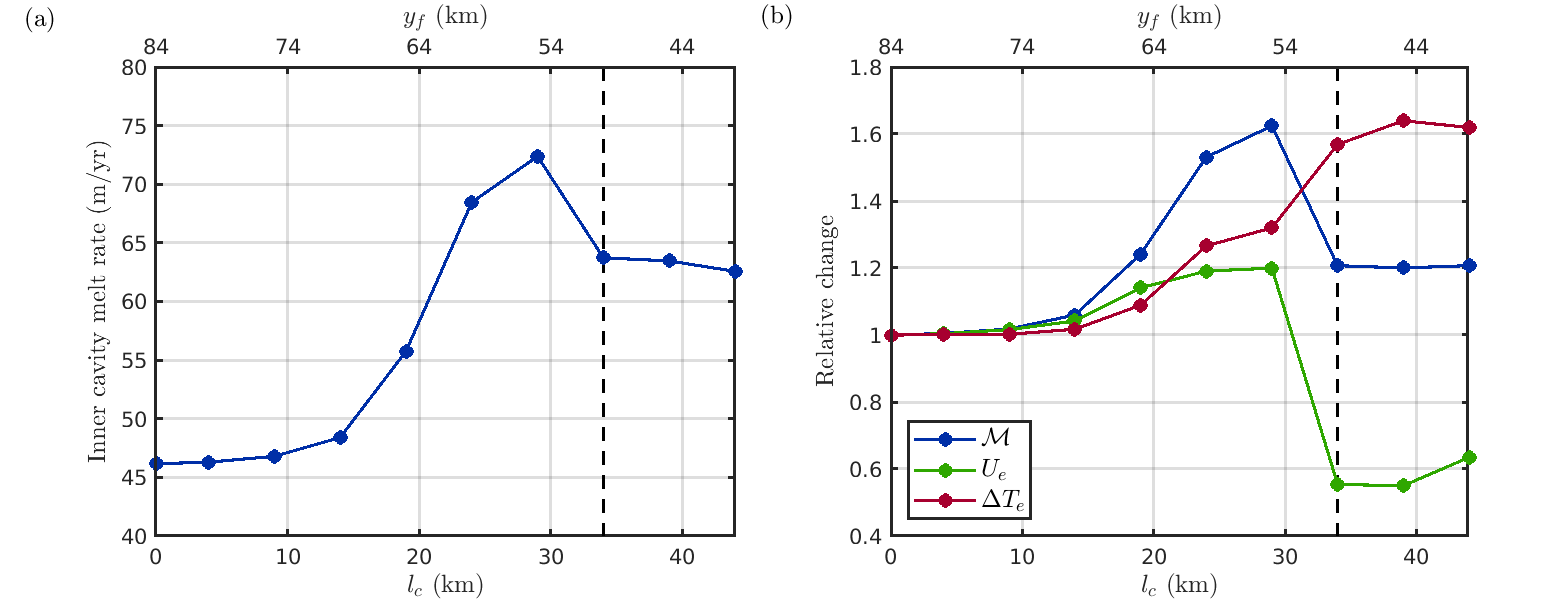
\includegraphics[width = \textwidth]{../make_figures/plots/figure4.png}
    \caption{(a) Mean inner cavity melt rate as a function of the calved length $l_c$. The black dashed line indicates the position of the ice front when it is located directly above the seabed ridge. (b) Velocity-thermal driving decomposition: decomposition of changes in inner cavity melt rate relative to the uncalved simulation into changes in boundary layer speed $U_e$ (green curve, equation~\eqref{E:MillgateDecompU}) and thermal driving $\Delta T_e$ (red curve, equation~\eqref{E:MillgateDecompDT}). The blue curve indicates the change in melting relative to the uncalved simulation (equation~\eqref{E:MillgateDecompMelt}). The green dashed line indicates the barotropic velocity effect $U_{be}$ (equation~\eqref{E:MillgateDecompUbaro}).  }
    \label{fig:figure4}
\end{figure}

%explain what the Millgate decomposition.
To understand the reasons for this variation in inner cavity melt rate with calving, it is instructive to return to equation~\eqref{E:MeltRateUdT}, which indicates that the melt rate is proportional to the product of the boundary layer velocity and thermal driving. We use this to investigate the relative roles of variations in both of these quantities in the changes to the inner cavity melt rate. To do so, we compute~\cite{Millgate2013JGROceans}
 \begin{align}
U_{e}(l_c) &=  \frac{\int_{\text{IC}}~u^*(x,y; l_c)~\Delta T(x,y;l_c = 0)}{\int_{\text{IC}}~ u^*(x,y; l_c = 0)~\Delta T(x,y;l_c = 0)}~\mathrm{d}x\mathrm{d}y, \label{E:MillgateDecompU}\\ \Delta T_{e}(l_c) &=  \frac{\int_{\text{IC}}~u^*(x,y; l_c=0)~\Delta T(x,y;l_c)}{\int_{\text{IC}}~ u^*(x,y; l_c = 0)~\Delta T(x,y;l_c = 0)}~\mathrm{d}x\mathrm{d}y, \label{E:MillgateDecompDT}
 \end{align}
where `IC' refers to the inner cavity (i.e. $y < 30$~km) and $u^*(x,y;l_c)$, $T(x,y,l_c)$, and $T_b(x,y,l_c)$ are the boundary layer velocity, ocean temperature, and local freezing temperature that emerge from the experiment in which the calving front is located at $y = l_c$, respectively. The quantities in~\eqref{E:MillgateDecompU}--\eqref{E:MillgateDecompDT} are compared, for a given calved length $l_c$, to the relative change in melting over the baseline simulation,
 \begin{equation}\label{E:MillgateDecompMelt}
   \mathcal{M}(l_c) =  \frac{\int_{\text{IC}}~u^*(x,y; l_c)~\Delta T(x,y;l_c)}{\int_{\text{IC}}~ u^*(x,y; l_c = 0)~\Delta T(x,y;l_c = 0)}~\mathrm{d}x\mathrm{d}y.
 \end{equation}
The quantities~\eqref{E:MillgateDecompU}--\eqref{E:MillgateDecompMelt} are plotted in figure~\ref{fig:figure4}b as a function of $l_c$.  Here, a melt response to calving that results exclusively from changes in the thermal driving would be indicated by indistinguishable blue and red curves, and a green curve that always takes the value one, while a melt response that results exclusively from changes in boundary layer velocity would be indicated by indistinguishable blue and green curves, and a red curve that always takes the value one. Henceforth, we refer to this comparison as a `velocity-thermal driving decomposition'. %(Note, however, that while the relative change in melt rate depends on the changes in velocity and thermal driving, this relationship is not linear.)

%what do these plots tell us about what is responsible for the changes?
The velocity-thermal driving decomposition (figure~\ref{fig:figure4}b) indicates that both changes in the boundary layer velocity and thermal driving play an important role in the melt response to calving (i.e. neither plays a dominant role).  When the ice front is located offshore of the ridge ($l_c < 25$~km), ice front retreat results in increases in both the boundary layer velocity and thermal driving; these increases are complimentary: they act in unison to increase the inner cavity melt rate as calving proceeds. When the calving front is retreated to sit above the ridge, the thermal driving effect increases further, while the velocity effect decreases sharply, corresponding to a significant reduction in the boundary layer velocity at this point. This reduction in cavity circulation outweighs the concomitant increase in thermal driving, leading to an overall reduction in the inner cavity melt rate. When the ice shelf is calved further beyond the ridge, both the thermal driving and boundary layer velocity effects are approximately constant.

%figure 6:  (a) row of melt rate (colours) and BSF contours, (b) zonal sections, (c,d) meridional sections
\begin{figure}
    \centering
    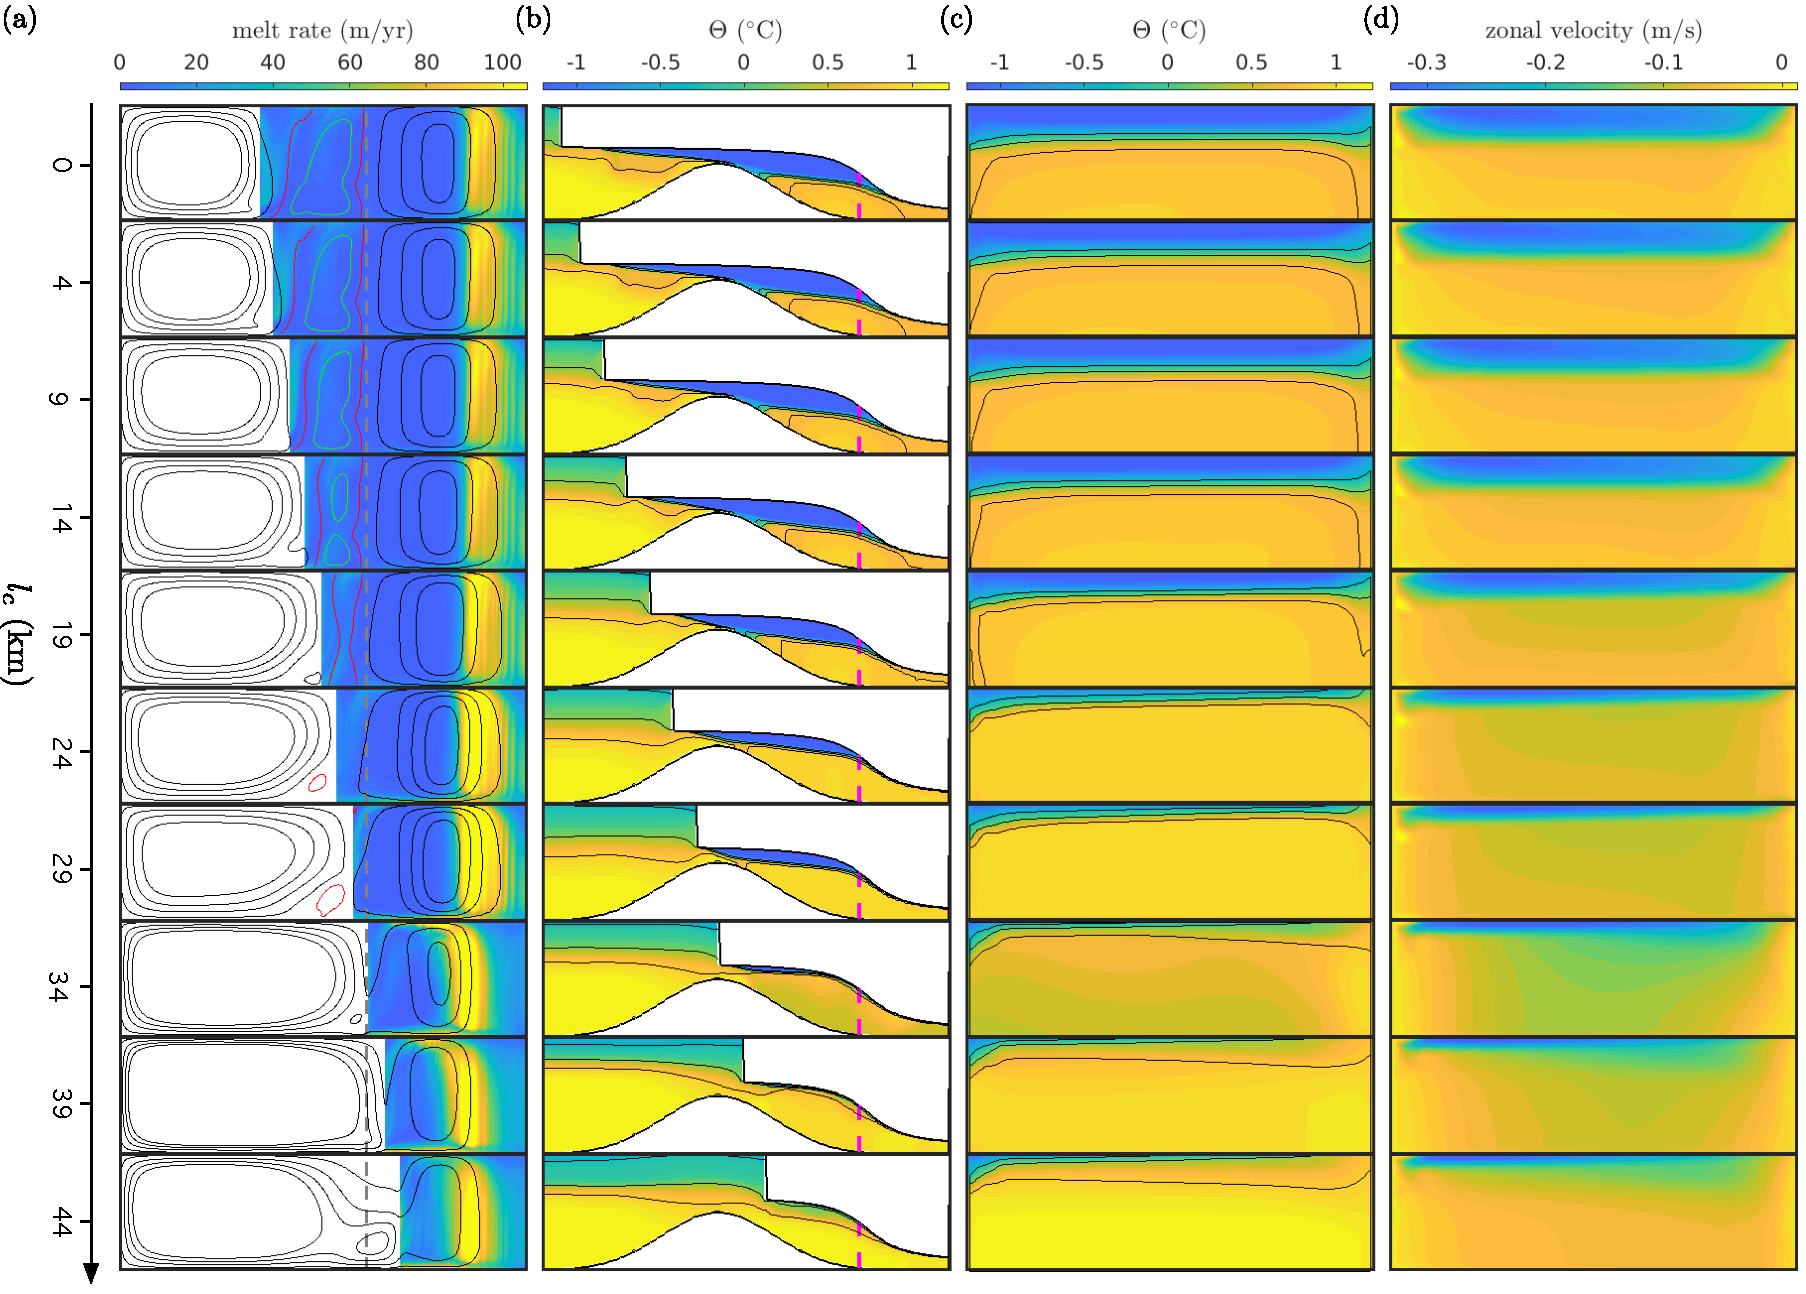
\includegraphics[width = 0.99\textwidth]{../make_figures/plots/figure5.pdf}
    \caption{(a) Contour plots of melt rate (colors) and barotropic stream function (contours, black at -0.1, -0.3, -0.5, and -0.7~Sv levels, magenta at the 0~Sv level, and green at the 0.05~Sv level) in the idealized simulations with $P = 600$~m and $W$ = 100~m. The calved length $l_c$ increases from 0~km in the first row to 44~km in the final row. The white sections indicate open ocean. (b) Contour plots of potential temperature $\Theta$ (colors) and salinity (contours, at levels 34.2, 34.4, and 34.6~PSU, i.e. as in figure~\ref{fig:figure3}) taken along the centreline of the domain (magenta dashed line in figure~\ref{fig:figure3}a). The white section at the top and bottom of each subplot indicate the ice shelf and seabed ridge, respectively. (c) Contour plots of potential temperature (colors) and salinity (contours, at levels 34.2, 34.4, and 34.6~PSU) along a zonal section located 20~km downstream of the grounding line [magenta dashed line in (b)]. (d) As in (c) with colors indicating the zonal velocity.  In each case, the color bar at the top of the column is appropriate for each row in the column. }
    \label{fig:figure5}
\end{figure}

%how can we understand what happens.
As mentioned, calving changes both the buoyancy flux and the water column thickness, with the latter having an impact only via barotropic dynamics. The impact of calving on the cavity circulation can thus be diagnosed by considering how the barotropic stream function changes with ice front retreat (figure~\ref{fig:figure5}a). Indeed, the boundary layer velocity  effect curve $U_e(\ell_c)$ follows a very similar pattern to the corresponding barotropic velocity effect curve $U_{be}(\ell_c)$ (figure~\ref{fig:figure4}b), which is computed as in~\eqref{E:MillgateDecompU} but with barotropic velocities:
\begin{equation}\label{E:MillgateDecompUbaro}
    U_{be}(l_c)  =  \frac{\int_{\text{IC}}~u_b(x,y; l_c)~\Delta T(x,y;l_c = 0)}{\int_{\text{IC}}~ u_b(x,y; l_c = 0)~\Delta T(x,y;l_c = 0)}~\mathrm{d}x\mathrm{d}y,
\end{equation}
Here, $u_b$ is the magnitude of the barotropic velocity. The agreement between $U_e(\ell_c)$ and $U_{be}(\ell_c)$ suggests, in terms of the melt response to calving, changes in barotropic velocity can be used a proxy for changes in boundary layer velocity, and the melt response to calving can be assessed from a barotropic perspective. %i.e. changes to the boundary layer velocity that result from changes in baroclinic flow that result from stratification are not important

There are two regimes we consider. In the first regime, the ice front is offshore of the ridge ($\ell_c < 30$~km); these cases are qualitatively similar to the uncalved case: the strong PV barrier provided by the ridge and ice draft remains in place and a topographically constrained cyclonic circulation is spun up inshore of the ridge. In particular, the large cyclonic PV that is generated in the inner cavity is mostly contained within this region. There is a weak anti-cyclonic circulation offshore of the ridge, with little barotropic flow between these two regions, i.e. across the ridge (figure~\ref{fig:figure5}a). Warm water is, however, able to flow across the ridge at the eastern boundary, where it is modified by mixing with the meltwater plume. As the ice front retreat proceeds, the meltwater volume becomes less prominent (figure~\ref{fig:figure5}b--c), so heat loss induced by mixing at the eastern boundary is therefore reduced and, as a result, the temperature of the warm water that enters the cavity increases (figure~\ref{fig:figure5}c). This is manifested as an increase in the thermal driving (figure~\ref{fig:figure4}b); the associated increase in meltwater flux strengthens the PV source in the inner cavity, driving a slightly stronger circulation (increase in $U_e$ in figure~\ref{fig:figure4}b), which itself enhances melting (figure~\ref{fig:figure4}a).

The second regime occurs when the ice front is located at or beyond the seabed ridge. As the ice front is retreated and nears the ridge, the two PV barriers (the ice front and the seabed ridge) approach one another, and the anticyclonic circulation in the outer cavity can no longer be sustained.  When the ice front is retreated to sit directly above the ridge crest, a significant barotropic flow (approximately 0.1~Sv) is able to cross the ridge (figure~\ref{fig:figure5}a), even though there is still a strong PV barrier provided by the water column restriction between ridge crest and ice draft. This is because the ice front induces vorticity in the water column through lateral shear, and this vorticity source allows the barotropic flow to break the $f/h$ constraint: the ice front is a `leaky' PV barrier. (Note that PV is able to leak across the ice front wherever it is located, but the effect of this on the system depends on where the front is located. If the ice front is located offshore of the ridge, the outer cavity absorbs any PV that is able to penetrate past the ice front, and the effect is not felt by the inner cavity, which is more than one Rossby radius away from the ice front. However, when the ice front sits on top of the ridge, this leaking occurs directly into the inner cavity, permitting a significant barotropic flow to cross the ridge.) The resulting barotropic flow across the ridge is far more effective at flushing the inner cavity than the overturning circulation that flushes it when the ice front is located further offshore; as a result, the inner cavity is entirely flooded with warm water (figure~\ref{fig:figure5}c). Although this means there is far more heat available for melting (thermal driving effect increases when the ice front coincides with the ridge crest, figure~\ref{fig:figure4}b), there is a significant reduction in the circulation because the melt driven cyclonic PV generated in the inner cavity is no longer constrained to stay in that region.

Once the ice front is retreated beyond the ridge, the strong PV barrier provided by the ridge crest and ice draft is relaxed. As in the picture painted above for the case that the ice front sits directly above the ridge crest, a significant barotropic flow is able to cross the ridge. The cavity is again efficiently flushed with warm water, resulting in strong thermal driving, but the inner cavity circulation is significantly reduced, compared to when the ice front is located just offshore of the ridge. Melt rates become independent of ice front position once the ice front has retreated beyond the ridge, indicating that the ridge only plays a role in the melt response to calving when it has an ice shelf overlying it and the ridge-draft gap is small enough, as will be shown.

In summary, when the ice front is located offshore of the ridge, the ridge-draft PV barrier prevents barotropic flow into the cavity and inner cavity flushing is weak. Reduced boundary mixing with meltwater as the ice front is retreated results in enhanced thermal driving and an elevated melt rate; in turn, this is associated with enhanced cavity circulation, and further increases in melt rate. However, ice front induced vorticity and the relaxation of this PV barrier as the ice front is retreated to the ridge (and beyond) permits barotropic flow across the ridge that efficiently flushes the inner cavity with warm water. Although this provides significant heat for melting, this is outweighted by reduced cavity circulation,  ultimately leading to a reduction in the inner cavity melt rate.

\section{Effect of Cavity Geometry on Melt Response to Calving}\label{S:Results:H}
%what are we doing here and why (briefly)
In the previous section, we analyzed how the inner cavity melt rate responds to ice front retreat, and identified the mechanisms responsible, in the case that the gap between the ice draft and ridge-crest is narrow. The strength of the topographic barrier that restricts warm water access to the inner cavity was identified as an important control on this response. In this section, we describe how this picture changes for larger values of $W$ (in particular, $W=150$~m and $W=200$~m), which lead to a weaker topographic barrier.

%how do melt rates change
%In figure~\ref{fig:figure6}, we plot the inner cavity melt rate and velocity-thermal driving decomposition as a function of the calved length $l_c$ are plotted in figure for both $W$ = 150~m and $W$ = 200~m. Comparison with the corresponding results for $W$=100~m (figure~\ref{fig:figure6}a) indicates that at larger values of $H$, the inner cavity melt rate is less sensitive to calving: the range of inner cavity melt rates reduces from approximately 27\mpryr for $W$=100~m to 10\mpryr and 7\mpryr for $H$=150~m and $H$=200~m, respectively. In addition, the peak inner cavity melt rate is reached when the ice extent is greater ($l_c$ is smaller) as the gap $W$ is reduced (approximately 29~km, 14~km, and 10~km for $W$=100~m, 150~m, and 200~m, respectively).


\begin{figure}
    \centering
    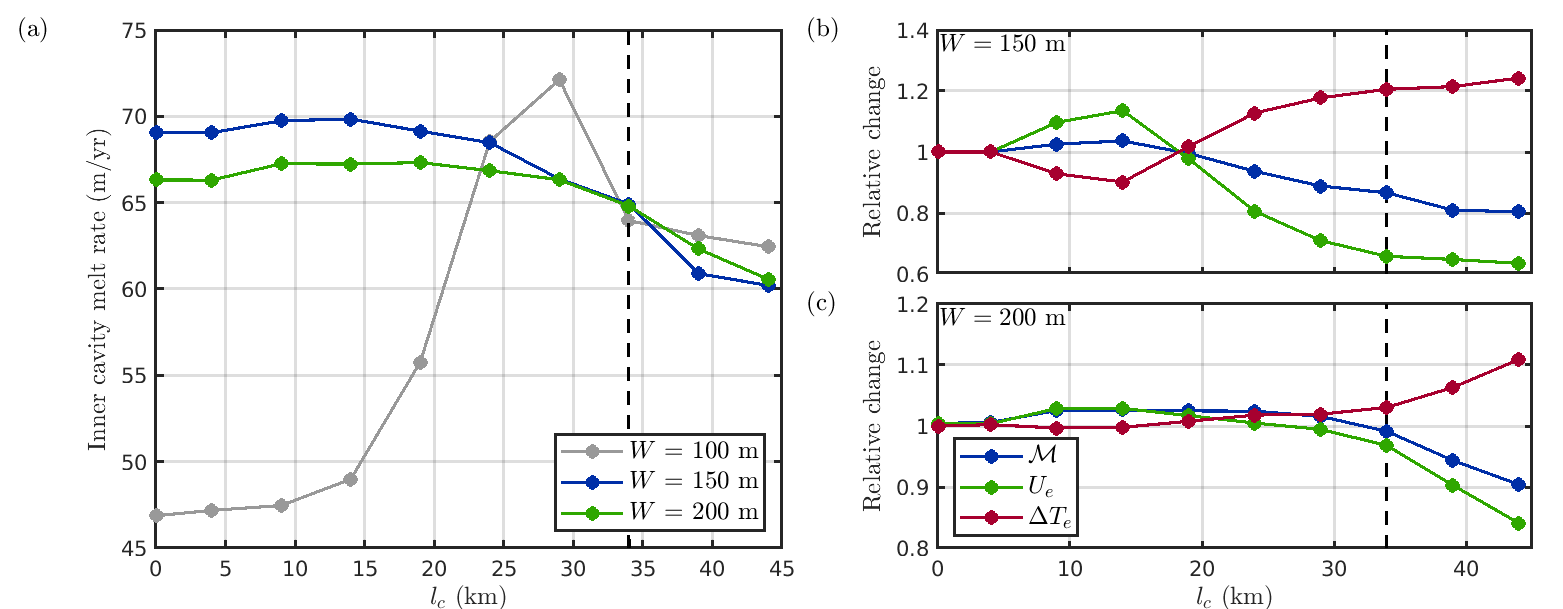
\includegraphics[width = \textwidth]{../make_figures/plots/figure6.png}
    \caption{(a) Inner cavity melt rate as a function of the calved length $l_c$ for $W$=100~m (grey, as in figure~\ref{fig:figure4}a), $W=150$~m (blue), and $W=200$~m (green).  (b)--(c) Velocity-thermal driving decomposition for (b) $W = 150$~m and (c) $W = 200$~m. In each plot, the black dashed line indicates the position of the ice front when it is located directly above the seabed ridge.}
    \label{fig:figure6}
\end{figure}

\begin{figure}
    \centering
    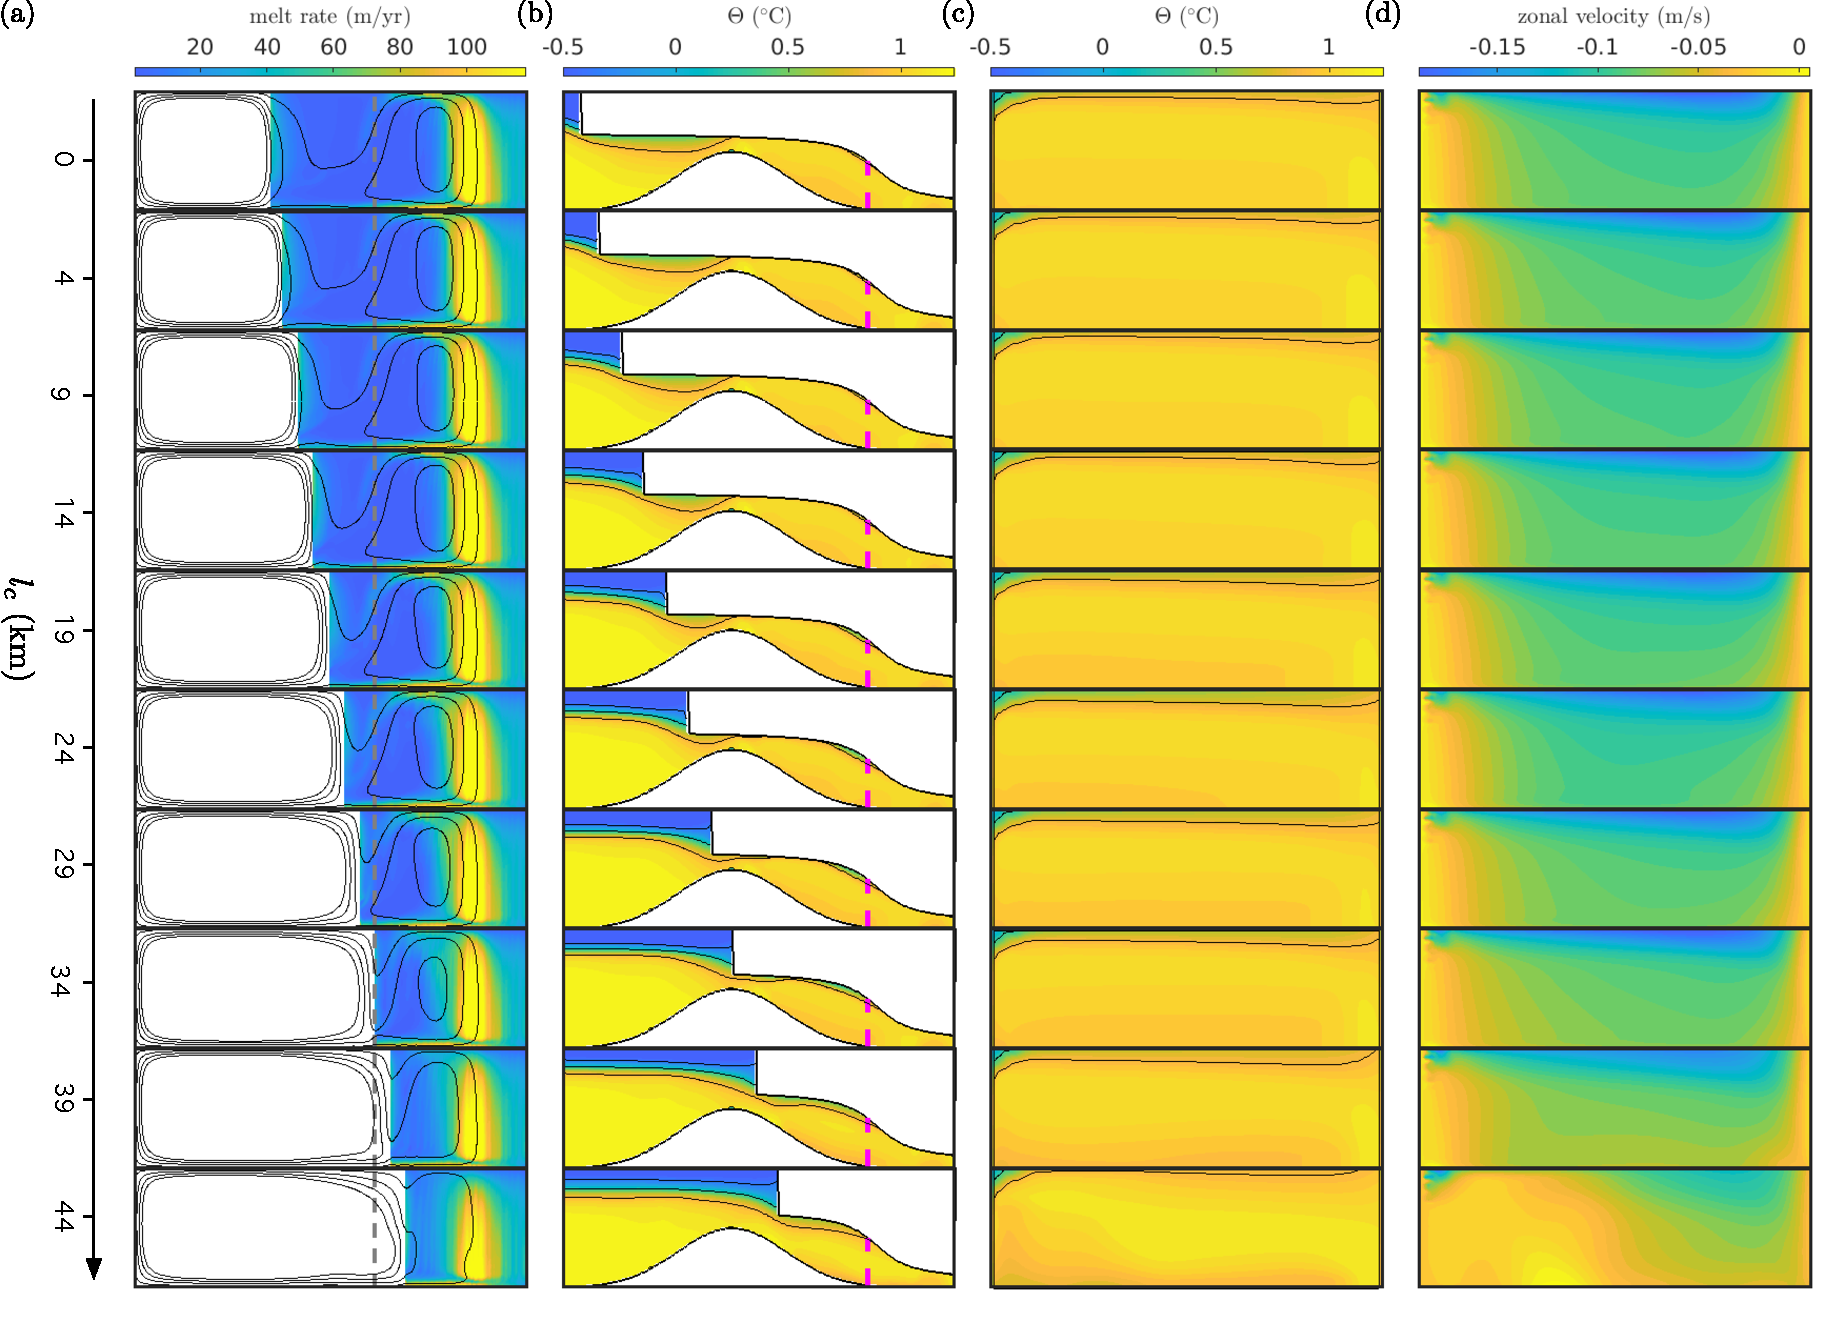
\includegraphics[width = \textwidth]{../make_figures/plots/figure7.pdf}
    \caption{Response of ocean characteristics to calving in the idealized experiments with $P=600$~m and $W=200$~m. This plot is as in figure~\ref{fig:figure5} for the experiment with $W=200$~m.}
    \label{fig:figure7}
\end{figure}


%what do we see
Mean melt rates as a function of calved length $l_c$ are plotted in figure~\ref{fig:figure6}a for both $W=150$~m and $W=200$~m in the $P = 600$~m case. We focus first on the $W = 200$~m case, which is characterized primarily by inner cavity melt rates that are largely independent of the ice front position. As before, we use the barotropic streamfunction to diagnose the behavior. This is shown, alongside zonal and meridional cross-sections, for the $W$=200~m case in  figure~\ref{fig:figure7} (the corresponding figure for $W = 100$~m is figure~\ref{fig:figure4}). Recall that, in the $W=100$~m case, two PV considerations are fundamental to the response: (1) when the ice front is offshore of the ridge, the ridge-draft PV barrier prevents barotropic flow into the cavity and inner cavity flushing is weak, but (2) ice front induced vorticity and the relaxation of this PV barrier as the ice front is retreated to the ridge, and beyond, permits barotropic flow across the ridge that efficiently flushes the inner cavity with warm water, but the associated increase in thermal driving is outweighed by a reduction in the inner cavity circulation. In the $W$=200~m case, however, the ridge-draft PV barrier is much weaker than in the $W$=100~m case, and barotropic flow across the ridge occurs even when the ice front is located offshore of the ridge (figure~\ref{fig:figure7}a); the regime in which barotropic flow across the ridge is entirely blocked, and melt-induced cyclonic PV is constrained within the inner cavity is never realized: for all values of $\ell_c$, PV is able to leak across the ridge, and the inner and outer cavities are dynamically connected. The system always behaves qualitatively similar to the highly calved regime for $W = 100$~m. The inner cavity is almost entirely flushed with modified CDW (figure~\ref{fig:figure7}b) and PV is not constrained to the inner cavity, regardless of the ice front position. Ice front retreat therefore has little effect in the $W = 200$~m case; in particular, this removes the tendency for both increasing temperature and circulation that we see in the $W$=100~m case before the ice front is retreated to the ridge. This invariance to ice front position also holds for larger ridge-draft gaps ($W>200$~m), a finding that is consistent with the results of~\citeA{DeRydt2014JGeophysResOceans}.

The $W = 150$~m case sits between these two situations (a strong response to calving for $W = 100$~m and a weak response to calving for $W = 200$~m). As in the $W = 100$~m case, there is a reasonable melt response to calving, although it is somewhat smaller in the $W = 150$~m case. In addition, inner cavity melt rate reaches a maximum when the ice front is located offshore of the ridge crest, and, further, the reduction in inner cavity melt rates for values of $\ell_c$ above that at which the maximum melt rate is attained results from a reduction in the inner cavity circulation that outweighs an increase in thermal driving. In contrast to the $W = 100$~m case, however, this scenario does not display a threshold-like behavior, where the inner cavity melt rate drops suddenly as the calving front reaches the top of the ridge. The weaker PV barrier in the $W=150$~m case means that, as in the $W = 200$~m case, the regime in which barotropic flow across the ridge is entirely blocked, is never seen; the threshold behavior, which occurs at the transition between the two regime, is therefore suppressed.


\section{Effect of Hydrographic Conditions on Melt Response to Calving}\label{S:Results:P}
Before moving on to assess how the inner cavity melt rate responds to calving in the realistic simulations, we briefly consider how the picture presented in the previous two sections changes depending on the choice of hydrographic forcing. Since we consider a constant ridge height, variations in the difference between the pycnocline depth and the depth of the ridge crest, which we expect to be a key driver of the quantity of warm water that is able to spill over the ridge and into the inner cavity, is captured here by variability in the value of $P$ (figure~\ref{fig:figure2}).

\begin{figure}
    \centering
    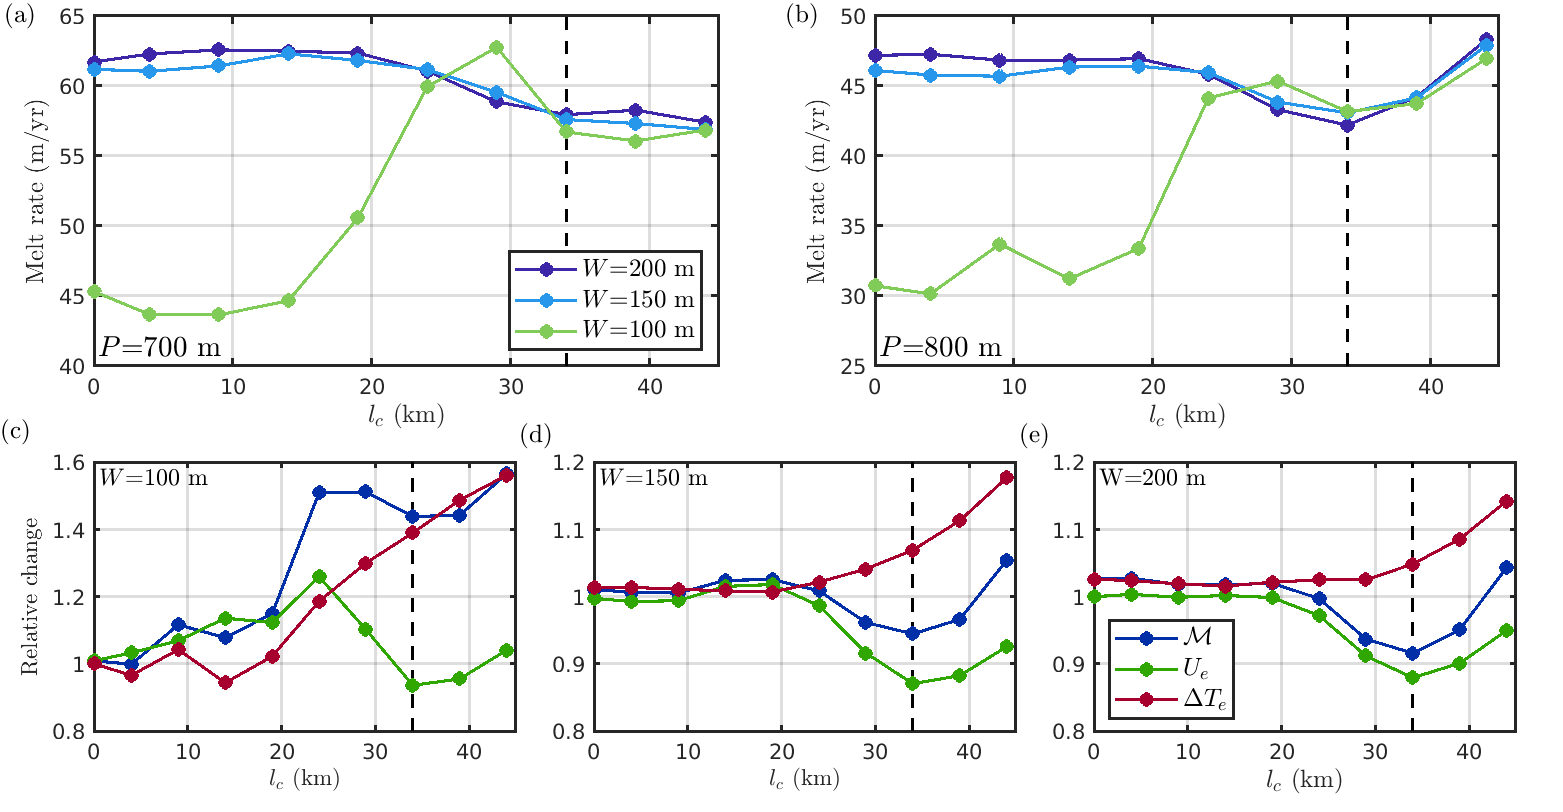
\includegraphics[width = \textwidth]{../make_figures/plots/figure8.png}
    \caption{(a)--(b) Inner cavity melt rate as a function of calved length $l_c$ in idealized simulations with (a) $P$=700~m and (b) $P$=800~m. Colors correspond to different values of $W$, as indicated by the legend in (b). The black dashed line indicates the location of the crest of the sea-bed ridge. The inset in (a) shows the sensitivity to the pycnocline position -- the ratio of the inner cavity melt rate for $P = 700$~m and $P = 800$~m [i.e. the ratio of the data represented by the green lines in (a) and (b))] -- as a function of the calved length $l_c$. (c)--(e) Velocity--thermal driving decompositions (as in figure~\ref{fig:figure4}) for the data shown in (b): (c), (d), and (e) correspond to the results for $W=100$~m, $W=150$~m, and $W=200$~m, respectively, as indicated.}
    \label{fig:figure8}
\end{figure}


% Introduce simulations with reminder of what they correspond to
The inner cavity melt rate and velocity-thermal driving decomposition for the experiments with $P=700$~m (hydrographic forcing as in the dashed profiles in figures~\ref{fig:figure2}b and c) and with $P=800$~m (dot-dashed profiles) are plotted in figure~\ref{fig:figure8}. The results for $P=700$~m are similar to those for $P=600$~m: for the narrowest gap ($W=100$~m), the inner cavity melt rate is sensitive to the ice front position, increasing rapidly as the ice front is retreated towards the ridge crest, before dropping off sharply when the ice front reaches it, and does not change under further ice front retreat. In addition, the sensitivity of melt rate response to calving reduces as the gap widens. A velocity-thermal driving decomposition for the experiments with $P=700$~m (not shown) is qualitatively similar to the $P=600$~m case discussed above: the melt response to calving can be explained by the interaction between changes in the amount of heat that is able to reach the inner cavity and the confinement of the cyclonic PV in the inner cavity. The similarity between the $P=600$~m and $P=700$~m cases is perhaps unsurprising when framed in terms of the relationship between the depths of the pycnocline and the ridge crest: in both cases, the CDW layer extends all the way to the top of the ridge (see figure~\ref{fig:figure2}) and thus the seabed ridge alone does not provide a significant barrier to CDW access to the inner cavity.

%results are different for P = 800 -- how?
In the $P=800$~m case, while the ice front is located offshore of the ridge, the melt rate is either constant or increases as the ice front is retreated, depending on the value of $W$ (figure~\ref{fig:figure8}b). A reduction in the ice-ocean boundary layer velocity is responsible for a drop in inner cavity melt rates as the ice front is retreated towards the ridge crest (figure~\ref{fig:figure8}c--e), as in the $P$=700~m and $P$=600~m cases. Beyond this point the $P$=800~m case differs from the $P = 600$~m and $P = 700$~m cases: calving taking the ice front beyond the ridge results in an \emph{increase} in the inner cavity melt rate (figure~\ref{fig:figure8}b), which is associated with a reversal of the reduction in boundary layer velocity (figure~\ref{fig:figure8}c--e) (i.e. the boundary layer velocity increases on average when the ice front is retreated beyond the ridge). The important difference in this case that the seabed ridge alone is able to provide a significant barrier that prevents warm water from reaching the inner cavity (the CDW layer in the outer cavity does not extend to the top of the ridge, see figure~\ref{fig:figure9}). As calving proceeds beyond the ridge, the thermal driving does not saturate (as in all the cases discussed above), but continues to increase, and the concomitant increase in glacial melt results in a stronger circulation (figure~\ref{fig:figure8}c).

\begin{figure}
    \centering
    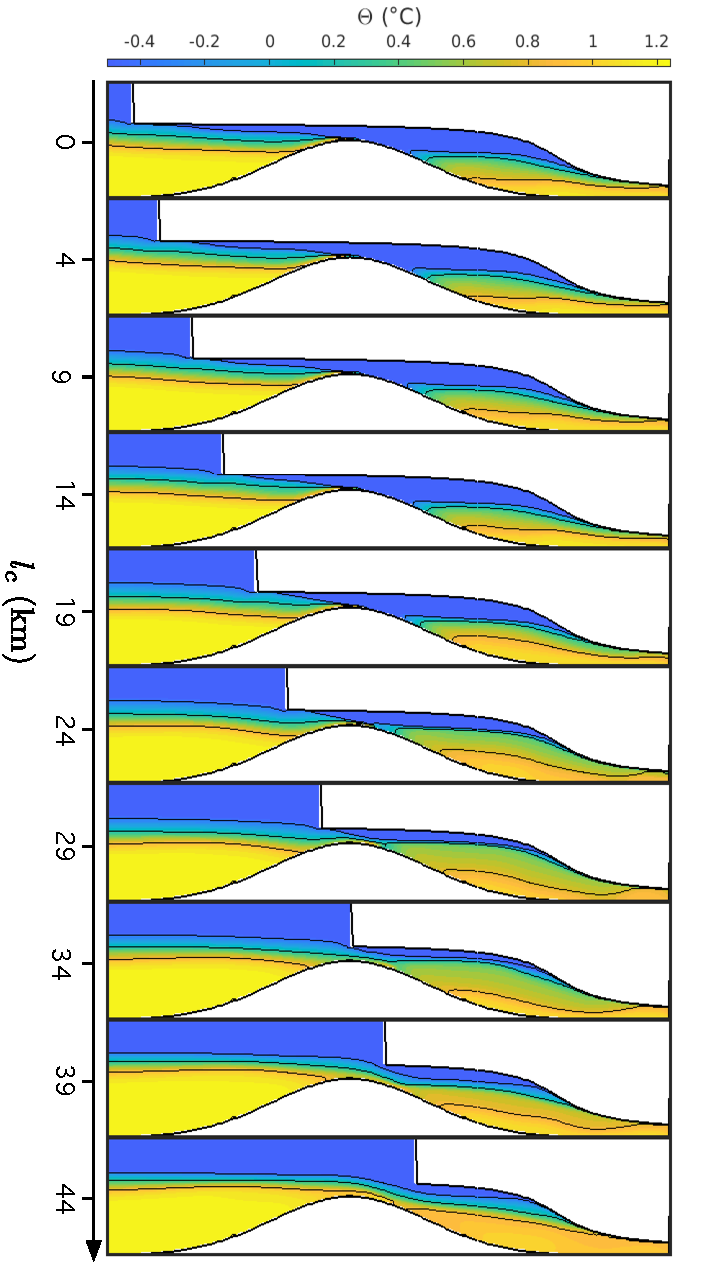
\includegraphics[width = 0.35\textwidth]{../make_figures/plots/figure9.pdf}
    \caption{Meridional cross sections for simulations with $P$=800~m, $W$=100~m. This plot is as in figure~\ref{fig:figure5}b for the simulation with $P$=800~m, $W$=100~m. }
    \label{fig:figure9}
\end{figure}

\section{Assessing the Melting Response of PIIS to Calving}\label{S:Realistic}
% intro to the section
The experiments described in \S\ref{S:Experiment}--\ref{S:Results:P} reveal how melt rates near the grounding line in idealized geometries with a uniform ridge-draft gap may respond sensitively to calving, depending on the thickness of the ridge-draft gap. These idealized experiments inform our understanding of similar experiments that are designed to assess the response of melt rates to PIIS calving. In this section, we describe these experiments, and present and analyze the results.

\begin{figure}
    \centering
    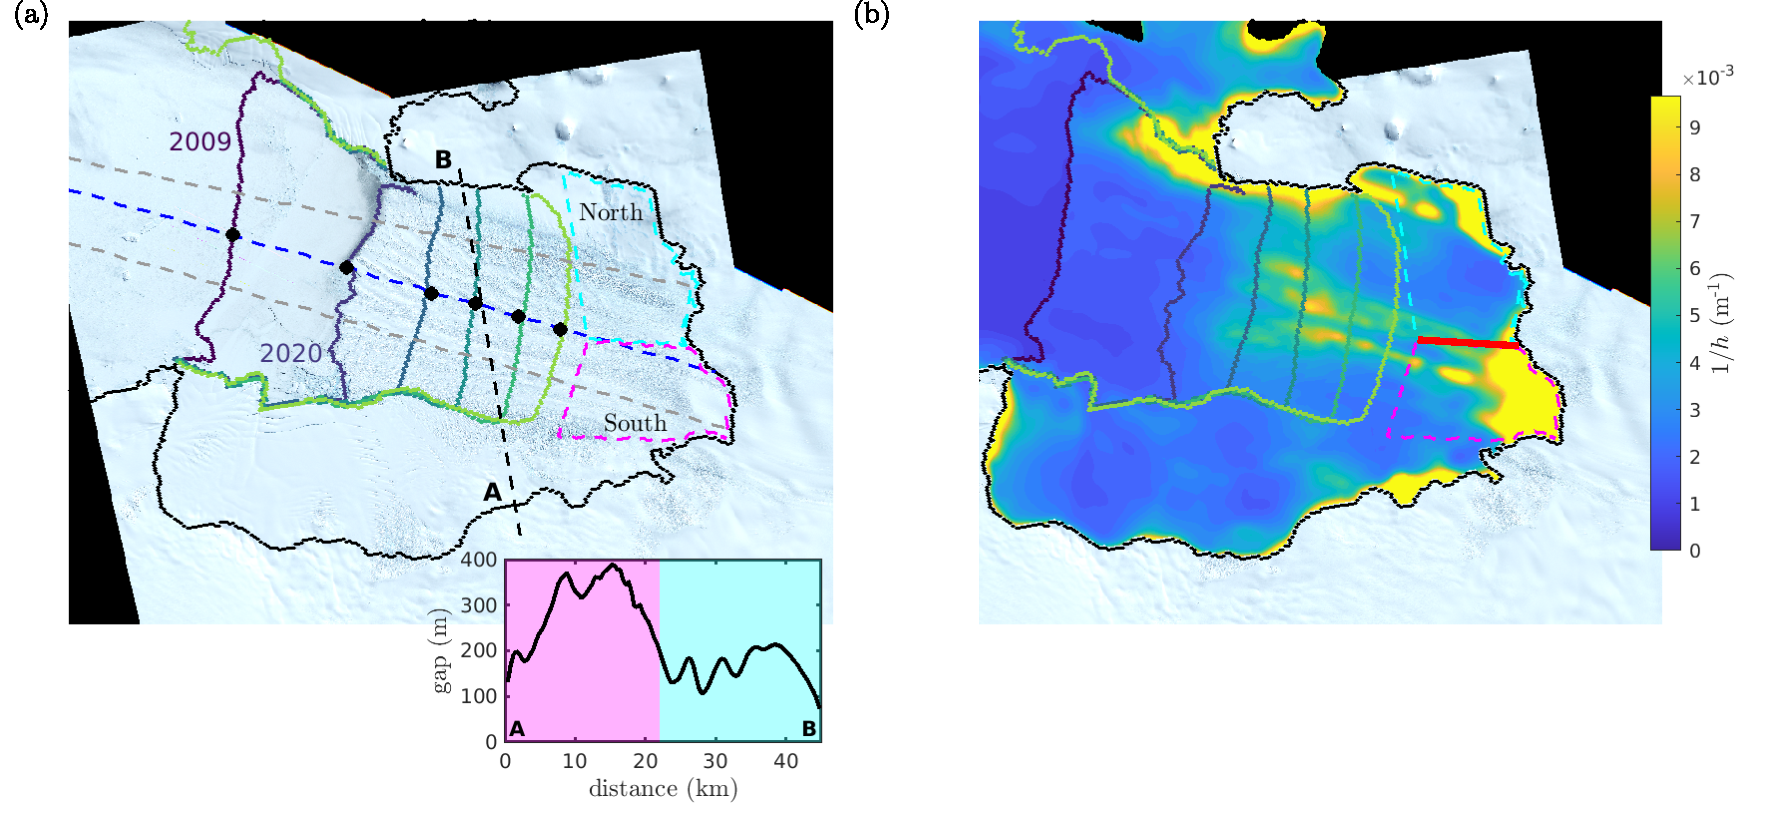
\includegraphics[width =\textwidth]{../make_figures/plots/figure10.pdf}
    \caption{(a) Ice front positions used in simulations to assess the response of the PIIS melt rate to calving. Each simulation corresponds to a different ice front position, indicated by the curves in the purple to green colormap; labelled dark purple and dark blue ice fronts correspond to the 2009 and 2020 front positions, respectively. The solid black line indicates the location of the 2009 grounding line from~\citeA{Joughin2010GRL}. The blue dashed line roughly indicates the centreline of the cavity, along which the calved length -- the difference between the ice front in the respective experiments and the 2009 ice front -- is measured, and the black dashed line approximately indicates the peak of the seabed ridge. The cyan (north) and magenta (south) boxes indicate the inner cavity regions considered in the experiments (see main text). Inset: plot of the (vertical) gap between the ridge crest and the ice draft, measured along the black dashed line in the main figure. Cyan and magenta shaded sections correspond to locations north and south of the blue dashed centreline, respectively. The background image is a Sentinel 2 mosaic from November 2020. (b) Inverse water column thicknesses $1/h$ used in these simulations. Ice front positions, inner cavity regions, and black dashed ridge crest are as in (a).  Note that the boundary between the inner cavity regions (solid red line) is approximately aligned with a region of locally enhanced $1/h$, indicating the presence of a potential vorticity barrier between the north and south inner cavity regions.}
    \label{fig:figure10}
\end{figure}

%Describe experiments
\subsection{Experiment Details}
Our experiments with a realistic setup are designed to assess the possible response of PIIS melt rates to calving in practice. To do so, we solve for the three-dimensional, semi-steady ocean circulation and associated melt rates simultaneously in a PIG cavity geometry [from~\citeA{Dutrieux2014Science}, and described briefly below], using the ocean model described in \S\ref{S:Experiment:Model}. We consider six different ice shelf topographies, each of which has a unique ice front position. The locations of these ice fronts are shown in figure~\ref{fig:figure10}: the first simulation (`2009' labelled curve in figure~\ref{fig:figure10}a) uses an ice shelf geometry that corresponds to PIIS in 2009~\cite{Dutrieux2014Science}. The second simulation (`2020' labelled curve in figure~\ref{fig:figure10}a) uses the 2009 ice shelf draft, but with a section of ice removed so that the ice front matches that obtained in 2020 (the ice front is determined from a Sentinel 2 mosaic of PIG). The four further simulations similarly use the 2009 ice shelf draft but with sections of fast flowing ice (i.e. within the shear margins) removed (figure~\ref{fig:figure10}). We stress that, as in the idealized experiments, the ice thickness, and thus grounding line position and ice shelf draft, at existing shelf locations remains the same in each experiment, and only the ice front position varies.

%how do we get cavity and draft
The sub-ice shelf cavity geometry we use is computed from the ice and seabed geometry, as described by~\citeA{Dutrieux2014Science}. Briefly, the ice shelf geometry is calculated from a 40~m-resolution digital elevation model (DEM) of the ice freeboard from 2008~\cite{Korona2009Photogrammetry}, which is adjusted with a constant median bias from observations obtained from the Autosub underwater autonomous vehicle~\cite{Jenkins2010NatureGeo}. The DEM assumes freely floating ice throughout the shelf, which may reduce its accuracy close to the grounding line. Over the continental shelf, the seabed geometry is well known from ship echo-sounding \cite{Dutrieux2014Science}, while in the cavity it is calculated from an inversion of gravimetry data and corrected point-wise using the median difference between the depth from the gravimetry inversion and the Autosub observations.

%model notes and calibration
We consider a single hydrographic forcing, corresponding to observed 2009 conditions in Pine Island Bay (dark grey line in figure~\ref{fig:figure2}b--c), to which the ocean is restored far from the ice shelf. All model parameters are as in the idealized experiments (described in \S\ref{S:Experiment:Model}). In particular, we take the drag coefficient in the three equation formulation of melting to be 4.5$\times10^{-3}$; this value is tuned so that the total meltwater flux in the simulation with the 2009 geometry (86~km\textsuperscript{3} year\textsuperscript{-1}) closely matches the estimated observed total meltwater flux for 2009 (80~km\textsuperscript{3} year\textsuperscript{-1}) \cite{Dutrieux2014Science}.

%gap is not uniform, but sort of split. Tell the reader what the different regions are.
As mentioned, the ridge-draft gap under PIIS is not uniform but varies from approximately 100~m at its narrowest to 400~m at its widest.  The ridge-draft gap (inset in figure~\ref{fig:figure10}) can be approximately partitioned into a northern section, where the gap is relatively thin, and a southern section, where the gap is relatively thick. A region of locally elevated $f/h$ running east-west (solid red line in figure~\ref{fig:figure10}b) meets the north-south aligned seabed ridge at the junction between these wide and narrow sections (see figure~\ref{fig:figure10}); this east-west aligned section extends all the way to the grounding line, partitioning the region inshore of the north-south aligned ridge into a northern inner cavity (cyan box in figure~\ref{fig:figure10}a) and a southern inner cavity (magenta box). The east-west aligned section of locally elevated $f/h$  provides a PV barrier between the two inner cavity regions, which are therefore approximately dynamically disconnected (figure~\ref{fig:figure11}a). In the following, we therefore evaluate the melt response to calving in the two inner cavity regions separately.

\begin{figure}
    \centering
    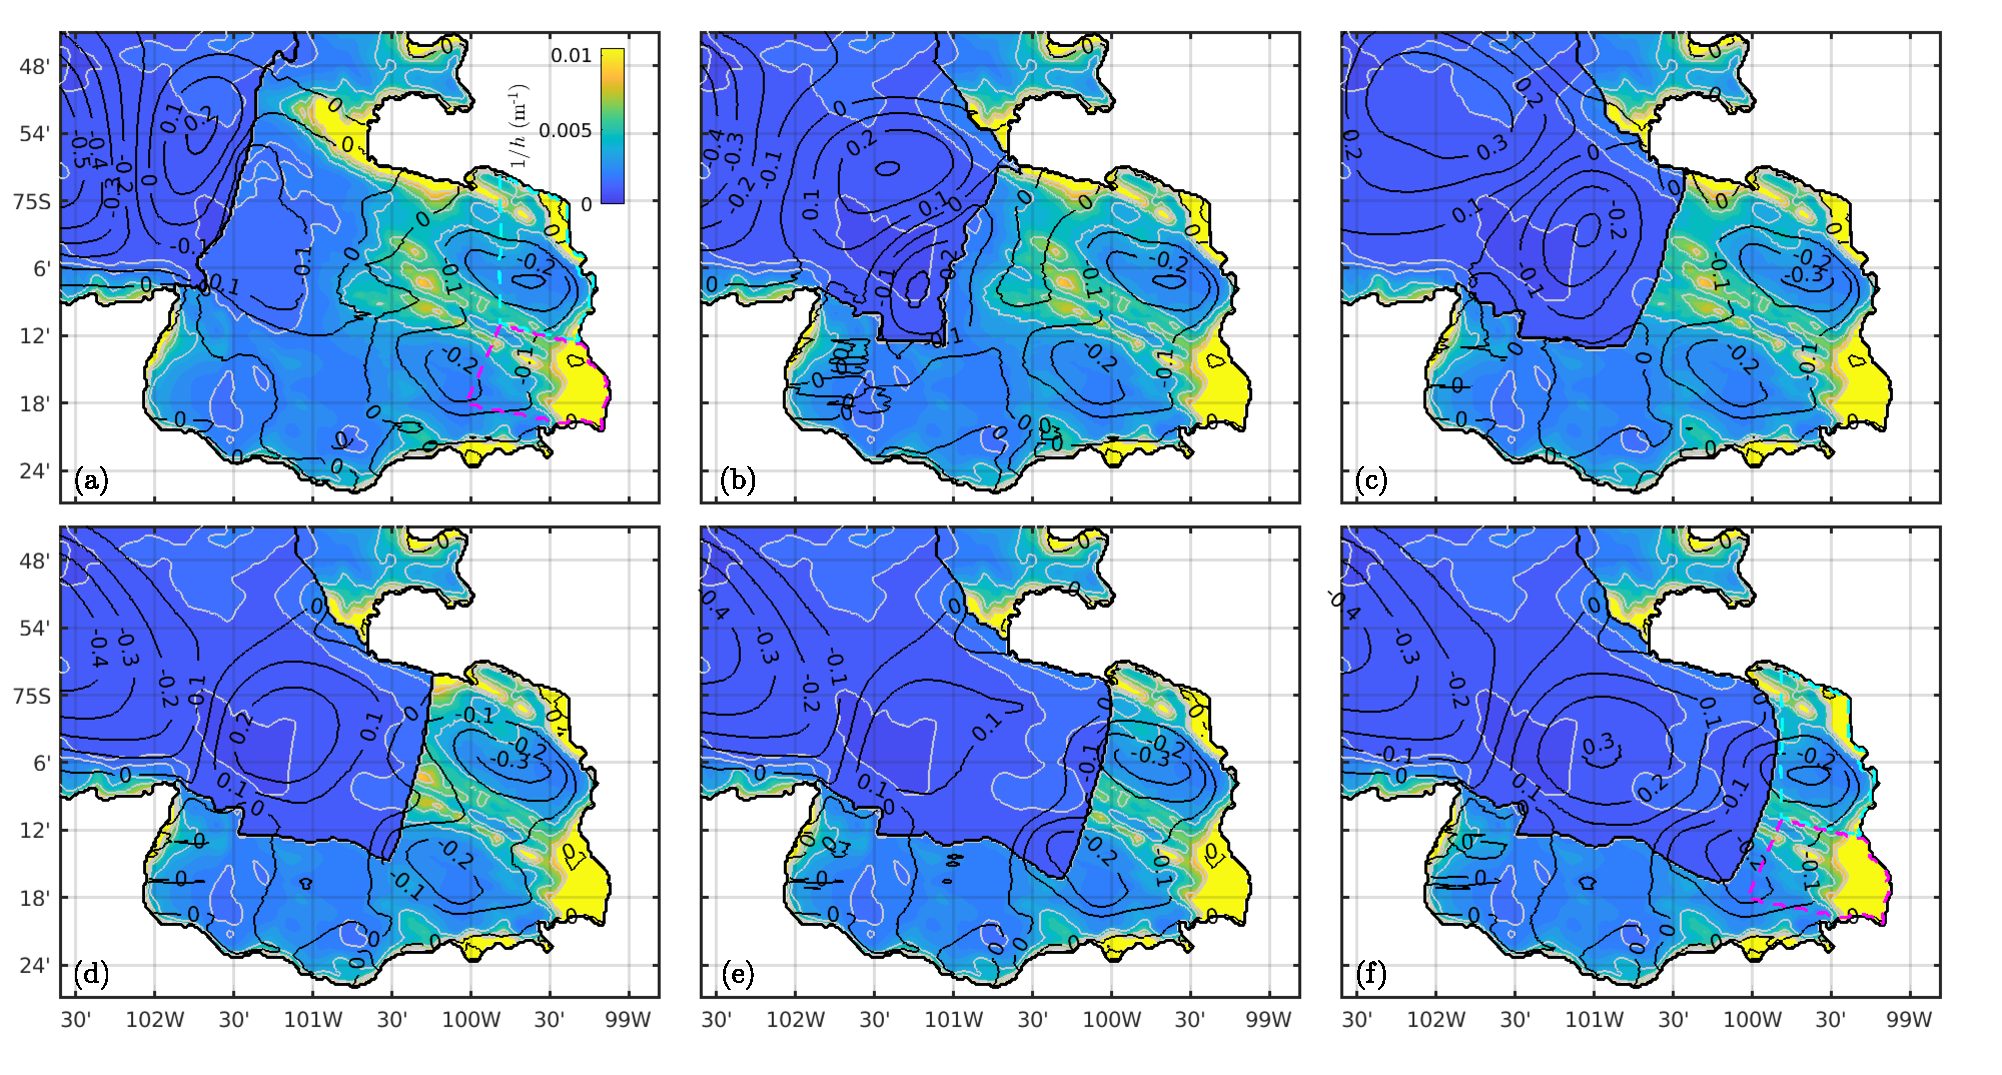
\includegraphics[width = \textwidth]{../make_figures/plots/figure11.pdf}
    \caption{Simulated barotropic stream function (labelled black contours) and inverse water column thickness $1/h$ (colors and grey contours at levels corresponding to 200, 400, 600, 800, and 1000~m water column thickness). Magenta and cyan dashed boxes in (a) and (f) indicate the extent of the north and south inner cavity regions, respectively.}
    \label{fig:figure11}
\end{figure}


\subsection{Results}

\begin{figure}
    \centering
    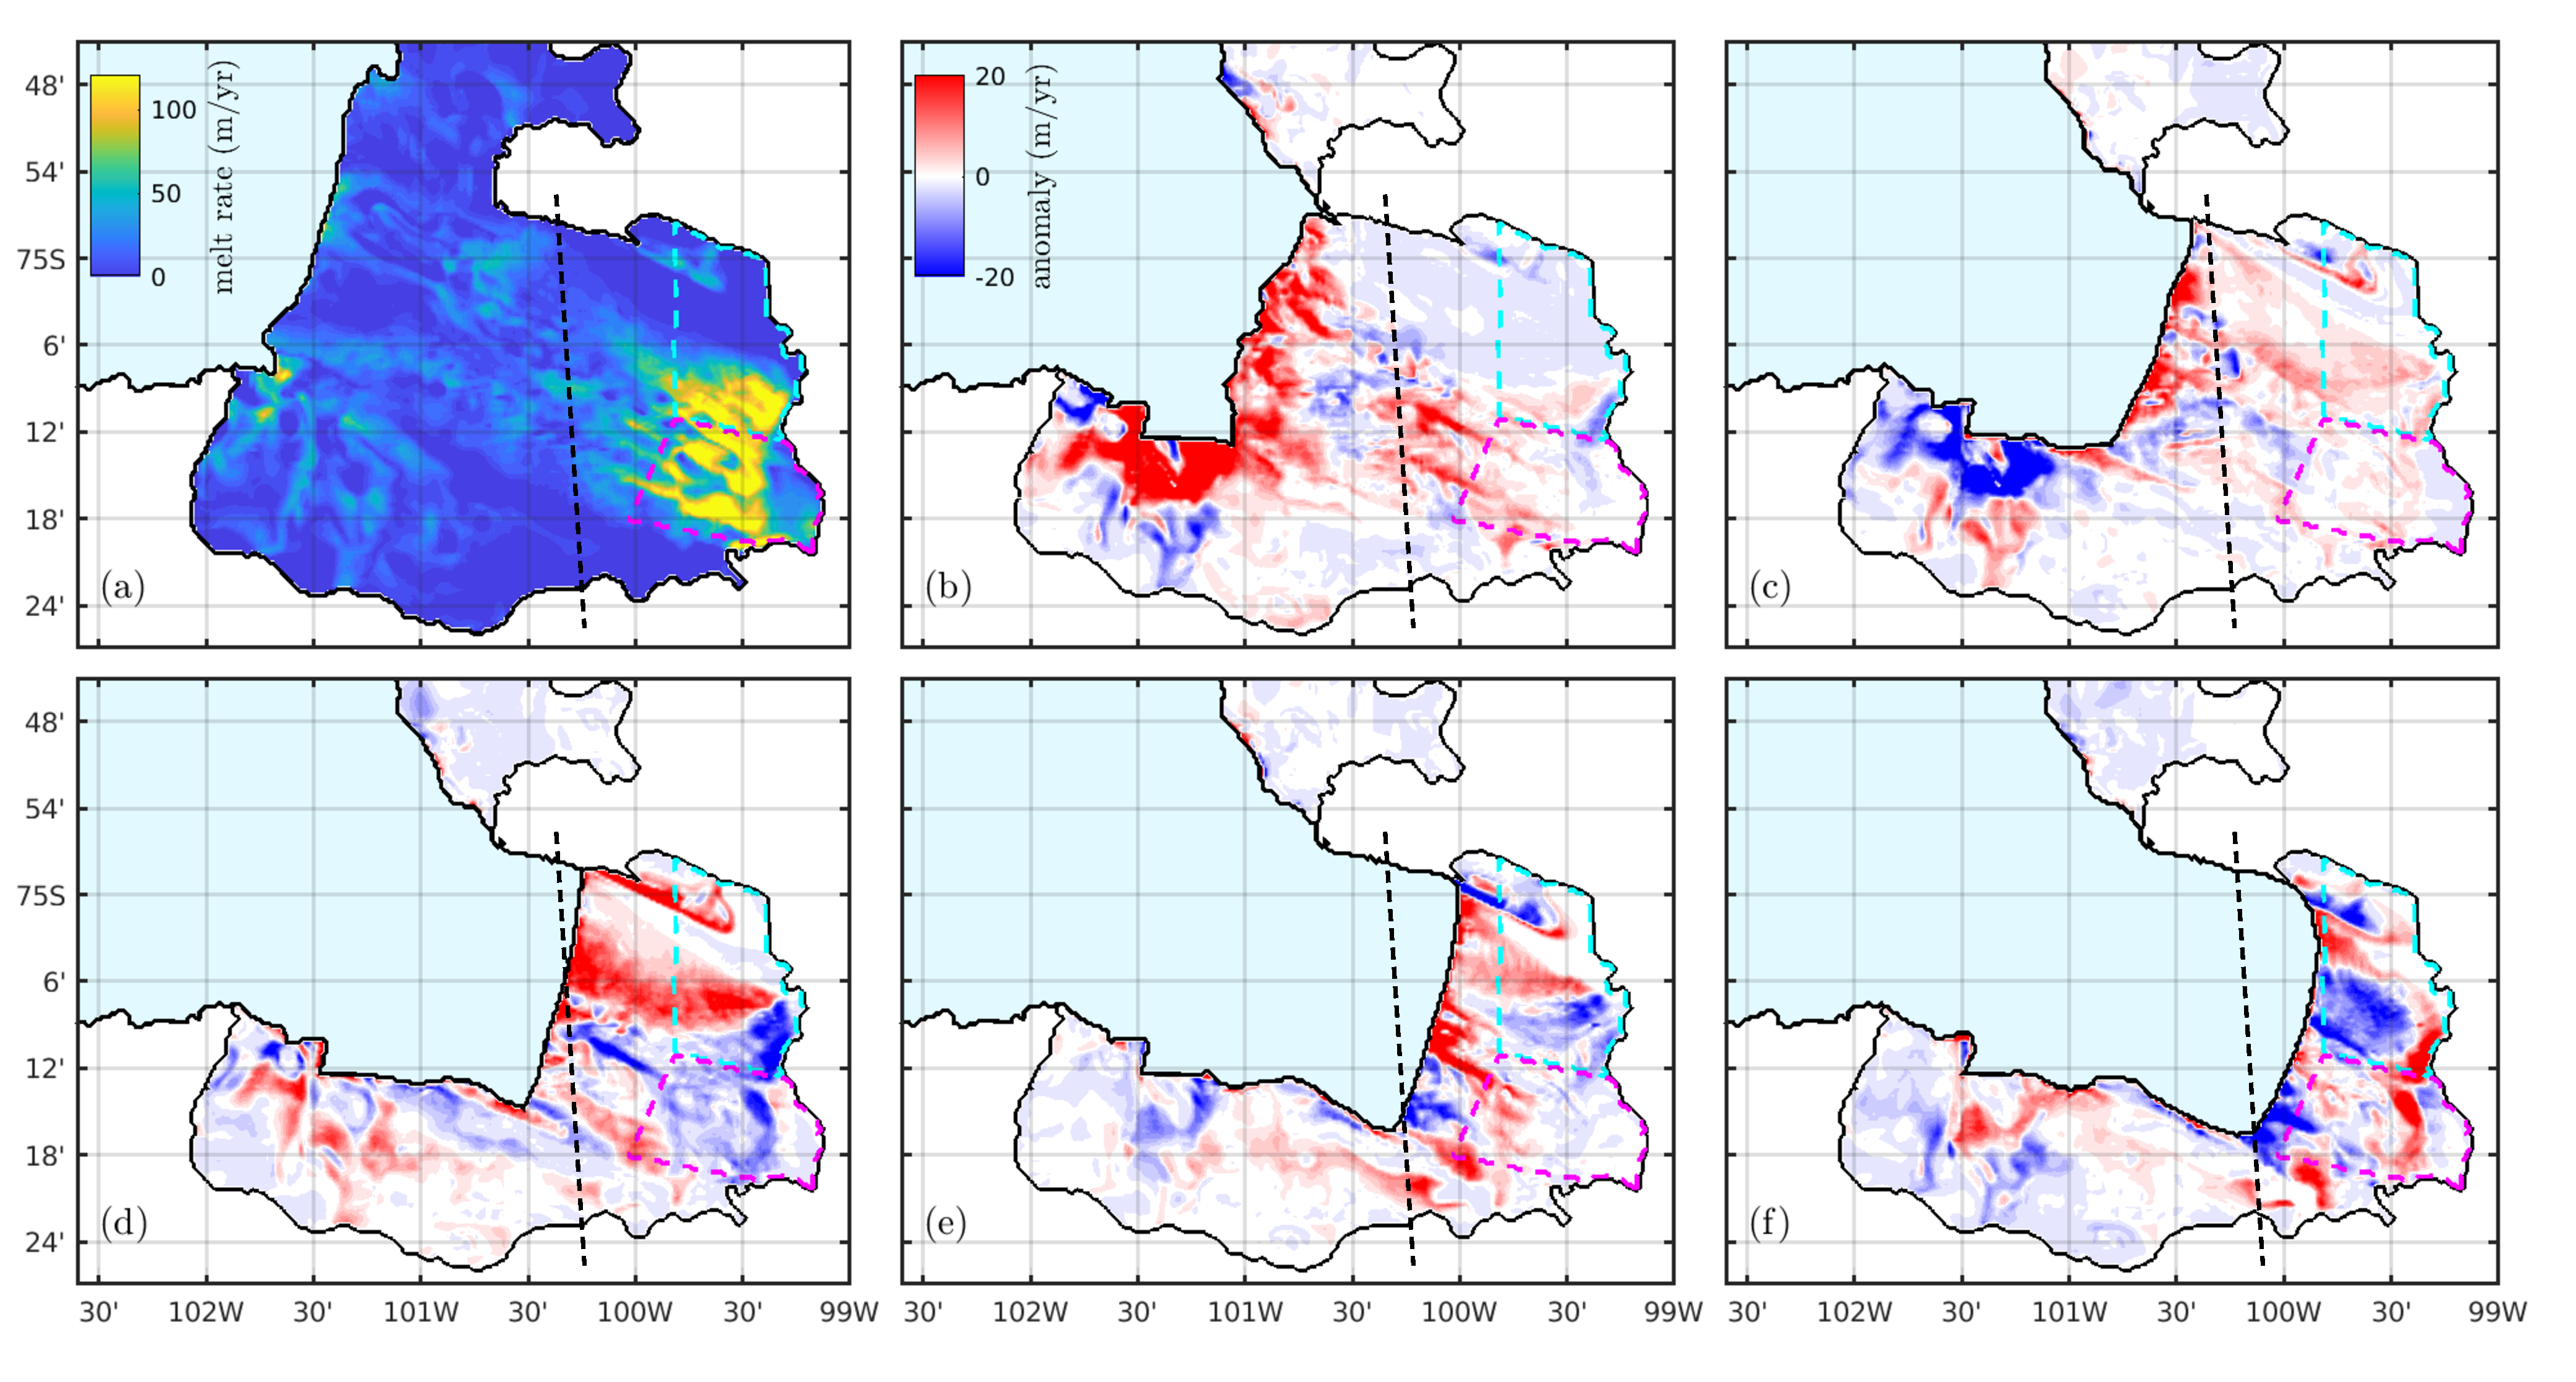
\includegraphics[width = \textwidth]{../make_figures/plots/figure12.pdf}
    \caption{(a) Simulated melt rate in the 2009 Pine Island geometry. Cyan and magenta dashed boxes [also in (f)] indicate the north and south inner cavity regions (see figure~\ref{fig:figure10}), where the highest melt rates are concentrated. (b)--(f) Non-cumulative melt rate anomaly in the simulations (i.e. measured relative to the previous panel). The colorbar in (b) is appropriate for each of (b)--(f). Note that melt rate anomalies in (b) are saturated to a maximum of 20~m~year\textsuperscript{-1} in the vicinity of the ice front (the maximum anomaly is approximately 30~m~year\textsuperscript{-1}). In each case, the ice shelf front and 2009 grounding line from \citeA{Joughin2010GRL}) are shown as a solid black line, and an estimate of the location of the ridge crest as a black dashed line.}
    \label{fig:figure12}
\end{figure}


%introduce simulations
Cavity circulation (figure~\ref{fig:figure11}a) and melt rates (figure~\ref{fig:figure12}a) in the uncalved (2009) simulation are qualitatively similar to the corresponding uncalved idealized simulations: melt rates are concentrated near to the grounding line, reaching a peak of approximately 120~m yr\textsuperscript{-1} several kilometers downstream of it, while remaining below 20~m~year\textsuperscript{-1} over the majority of the shelf. This pattern of simulated melt rates under PIIS is consistent with observations~\cite{Dutrieux2013Cryosphere} and other numerical simulations of cavity circulation under PIIS~\cite[for example]{Heimbach2012AnnGlac}. A cyclonic circulation spins up within each of the inner cavity sections, as well as in the outer cavity between the seabed ridge, and in the open ocean offshore of the ice front. Barotropic stream function contours largely follow the contours of constant water column thickness (figure~\ref{fig:figure11}).

Figure~\ref{fig:figure12}b--f show the non-cumulative melt rate anomalies for the other five experiments. To be explicit, non-cumulative here means that red (blue, respectively) locations on these maps indicate areas in which the melt rate increases (decreases) when the ice front is retreated from its position in the next largest ice shelf, i.e. changes in melt are shown relative to the previous experiment in the series, rather than relative to the first (2009) simulation.

%2009--now: large anomalies at the front
When the ice front is retreated from its 2009 position to its 2020 position, melt rates within 10~km of the ice front increase significantly (figure~\ref{fig:figure12}b). This is attributed to high velocities associated with upwelling at the new ice shelf front, as well as the formation of a reasonably strong gyre in the newly exposed open ocean which is covered by the ice shelf in the 2009 configuration (figure~\ref{fig:figure11}b). This double gyre pattern is qualitatively similar to observations taken in PIB in 2020~\cite{Yoon2021}. The gyre adjacent to the shelf results in a strong circulation along the front, which itself acts as a dynamic barrier to flow, as well as providing a freshwater source to further enhance the flow. Melt rates in both inner cavity regions do not change significantly when the ice front is retreated from its 2009 position to its 2020 position: the average melt rate in the northern and southern boxes increases by approximately 0.2~m~year\textsuperscript{-1} and 1.2~m~year\textsuperscript{-1} respectively (figure~\ref{fig:figure13}a, c).

%Qualitative descriptions of melt anomalies: (a) characterized by complex patterns, (b) only see significant changes when calving beyond the ridge (large positive anomaly in the northern shear margin which might be important for stability), (d) melt rates decrease when ice front has retreated significantly (this is a lead in to the qualitative analysis of fig 12)
Melt rates in the simulations with ice fronts retreated beyond the 2020 position display complex patterns of change, which include large regions of both positive and negative anomalies (figure~\ref{fig:figure12}c--f). Melt rates do not change significantly in the first `future' scenario, in which the ice front is still located some way offshore of the ridge, in qualitative agreement with the idealized results. Melt rates in the vicinity of the northern shear margin increase dramatically when the ice front is retreated to a position that sits (approximately) above the seabed ridge (figure~\ref{fig:figure12}d), and this region of enhanced melt rates extends almost all the way to the grounding line. With the ice front immediately above the seabed ridge, the outer cavity region no longer exists; this is reminiscent of the idealized results in which there is a qualitative change in the behavior when the outer cavity disappears and the only remaining regions of closed $f/h$ space are the inner cavity and the open ocean.  %The barotropic component of flow is able to penetrate under the southern shear margin because a depression in the sea bed there (red circle in figure~\ref{fig:figure11} results in a reduced water column thickness discontinuity that can be overcome; this supports our earlier assertion that flow under PIIS is essentially controlled by PV constraints.
This large melt rate anomaly is accompanied by a change in the direction of the circulation in the open ocean (figure~\ref{fig:figure11}d), which is consistent with conservation of PV: prior to retreat beyond the ridge, melt water leaving the cavity did so offshore of the ridge, where the water column thickness increases in the direction of flow; in this case, conservation of PV requires flow to be diverted clockwise. However, when the ice front is located inshore of the ridge, the water column thickness reduces at the ice front; in this case, conservation of PV thus requires flow to be diverted anti-clockwise, setting up an anti-cyclonic circulation in the embayment.

\begin{figure}
    \centering
    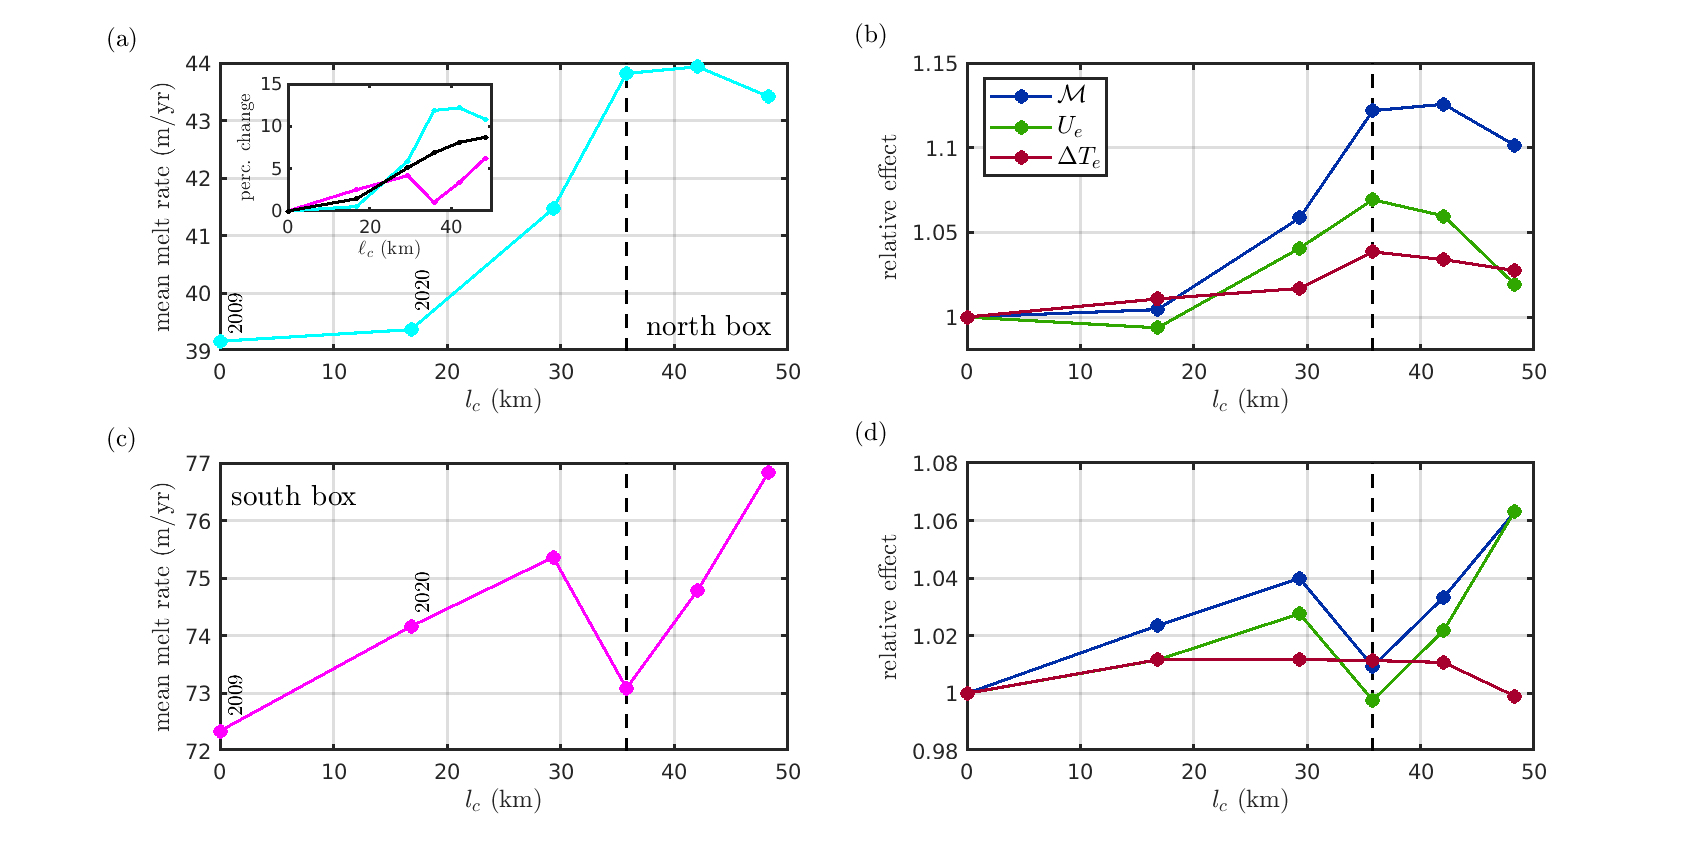
\includegraphics[width = \textwidth]{../make_figures/plots/figure13.png}
    \caption{(a), (c) Average melt rate as a function of calved length $l_c$ in simulations using a PIG geometry. Plots (a) and (c) correspond to the north and south regions of the inner cavity, respectively (cyan and magenta boxes in figure~\ref{fig:figure10}). The calved length $l_c$ is the distance measured along the blue dashed line in figure~\ref{fig:figure10}a, taken relative to the 2009 ice front position (purple curve in figure~\ref{fig:figure10}a). (b), (d) Velocity-thermal driving decomposition for the changes in melt rate shown in (a) and (c), respectively. As indicated by the legend in (b), blue, red, and green curves correspond to simulated changes $\mathcal{M}$, velocity effects $U_e$, and thermal driving effects $\Delta T_e$, respectively. In each of the plots, the black dashed line approximately corresponds to the calved length when the ice front sits approximately above the ridge crest.}\label{fig:figure13}
\end{figure}

%these qualitative observations sort of agree with the mean melt rate plots
We show in figure~\ref{fig:figure13}a and c the mean melt rate as a function of calved length for the north and south inner cavity regions, respectively. In the northern region, mean melt rates remain approximately constant until the ice front approaches the seabed ridge, where they increase sharply, before remaining approximately constant as the ice front is retreated further. In the southern box, melt rates are less variable (in terms of percentage change), but the overall trend is that the melt rate increases while the ice front is located downstream of the seabed ridge, before dropping temporarily when the ice front is retreated to the ridge and subsequently increasing again.


%northern box 'hides' behind a narrow gap -- make comparison with the narrow idealized case
Our interpretation of these results is guided by the idealized simulations presented in \S\ref{S:Baseline}--\ref{S:Results:P}. In the northern box, the inner cavity is shielded by a relatively narrow gap between the seabed ridge and the ice draft (inset of figure~\ref{fig:figure10}a), and the change in melt rates with calving behaves in a qualitatively similar way to idealized results with narrower gaps ($W\leq150$~m). A velocity-thermal driving decomposition of these changes in melt rates (figure~\ref{fig:figure13}b) indicates that, as in the corresponding idealized case, both increases in thermal driving and velocity contribute to the increases in melt rate with calving while the ice front is located offshore of the ridge, and that a reduction in the boundary layer velocity is responsible for the decrease in melt rates when the ice front is retreated beyond the ridge. This suggests that the enhancement in melt rates with calving while the ice front is located offshore of the ridge is driven by increased heat reaching the inner cavity and a concomitant increase in meltwater flux and thus circulation strength. As in the idealized case, when the calving front reaches the ridge, the trend of increasing melt rate with calving is reversed, although in this case that is observed as a saturation of the, rather than a strong reduction, as in the idealized case.

%In the idealized case, however, the effect of a reduction in the boundary layer velocity was stronger, and the decrease in melt rate larger, than in this realistic case; we attribute this difference to the splitting of a connected domain into two sub-regions, and the particular complexities of the realistic cavity.

%southern box 'hides' behind a wide gap -- make comparison with the wide idealized case
The southern inner cavity region sits inshore of a relatively wide gap between the seabed ridge and the ice draft (figure~\ref{fig:figure10}). As was the case for idealized simulations with wide gaps ($W\geq200$~m), the mean melt rate is far less sensitive to the ice front position than it is with a narrow gap (i.e. for the northern box): the difference between the minimum and maximum melt rates in the southern box is approximately 6\%, which is almost half of the corresponding value in the northern box. This invariance under calving suggests that the inner cavity is flushed with warm water in each simulation; calving, which acts primarily to increase heat content in the inner cavity, has little effect.

%The superimposed trend (increasing melt rates, except for a drop when the ice front is located on top of the ridge associated with a reduction in velocities, see figure~\ref{fig:figure13}) is reminiscent of the results of the idealized simulations with a lower pycnocline (see figure~\ref{fig:figure8}(b)--(e)); by drawing an analogy to the idealized results, this suggests that the southern cavity is not entirely flooded with warm water, and ice front retreat continues to increase stratification, even after the ice front has been retreated beyond the ridge.


\section{Discussion}\label{S:Discussion}
%loss of area led to increase in speed, but did it also lead to increase in melting which might promote further buttressing loss? Yes at the ice front, but not at GL or shear margins. This suggests negative feedback
The results of the previous section suggest that the recent calving of PIG has not lead to increases in melting in either the shear margins or near the grounding line, which are particularly important for buttressing of the grounded ice sheet~\cite{Furst2016NatureClimCh, Reese2018NatureClimCh}. Therefore, we do not expect that further buttressing losses associated with increased shelf melting will take place as a result of the recent calving. This lack of response might represent a negative feedback on ice shelf loss: the recent calving led to an acceleration of the grounded ice~\cite{Joughin2021ScienceAdv}, and thus an increase of the flux of ice into the shelf; to maintain a constant ice shelf mass balance, melting must therefore increase. The lack of increase in melting after the 2020 calving therefore shifts the shelf mass balance towards positive, i.e. it promotes regrowth of the ice shelf.

However, if calving maintains its pace since 2015, the situation in which the ice front sits above the ridge-crest will be realized in the mid 2020s. Large melt anomalies occur at both the shear margin and near the grounding line when the ice front is retreated to the ridge crest. Assuming that calving fluxes remain unchanged, if the increase in mass loss due to melting after calving to the ridge crest is larger than the resulting increase in flux across the grounding line (that results from buttressing losses after calving), the ice shelf mass balance will reduce, i.e. a calving event that takes the ice front to the ridge crest may lead to further mass loss, representing a positive feedback on ice shelf mass balance. It is important to stress that these feedback arguments are qualitative: investigating the detailed response of the ice shelf mass balance to calving event requires the use of a coupled ice-ocean model, and is beyond the scope of this study.
%recent speed up leads to thinning and thus retreat, but also acceleration, which needs an increase in melt to balance. We find no increase in melt, so melt response (i.e. no response) will help to promote shelf regrowth. However, assessing this in detail needs use of a coupled ice ocean model.



%In future melt rates generally increase in future, but changes are smaller than idealized results suggest (why?)
The magnitude of changes in melting with calving in the southern cavity (for which the offshore ridge-seabed gap is wide) in our realistic simulations are similar to corresponding idealized simulations (i.e. very small). For the northern section of the cavity (narrow ridge-seabed gap), although the changes are qualitatively, their magnitude is smaller than the corresponding idealized experiments predict. We attribute this difference to the complexities of the ice draft and seabed in the realistic simulations, and as well as our splitting of the inner cavity into two subsections, which relies on the assumption that they are entirely dynamically disconnected. Although a strong PV barrier exists between them, some flow is able to cross this barrier, providing a connection between the two regions. This inner cavity decomposition is also a convenient tool that permits us to account for some of the effect of the inhomogeneity in ridge-draft gap along its length, but further work is required to fully understand the role variations in the ridge-draft gap in controlling warm water access to the inner cavity.

In addition, the sensitivity to cavity geometry identified in the idealized simulations means that the observed response may in fact be somewhat different to that predicted here: if, for example, the ridge-draft gap is, in practice, smaller than that used in our realistic simulations (there are reasonable uncertainties in the ice draft and bathymetry beneath the shelf), the melt response to calving might be significantly larger. Furthermore, the ice draft is not static but varies dynamically; advection of thicker (thinner, respectively) sections of the ice shelf to the ridge crest would be expected to narrow (widen) the ridge-draft gap and thus increase (decrease) the sensitivity of melt rates to calving. If we ignore the locations of changes in melting, and focus purely on mean melt rates, our idealized simulations suggest a melt-gap feedback for any ice front position offshore of the ridge: if the ice front is located offshore of the ridge, the melt rate is increasing with $W$ for all values of $P$, and this reduction in the gap width will promote a reduction in melt rates; the resulting thickening of the ice shelf is then expected to lead to a further reduction in the ridge-draft gap and thus melt rates. The vice versa case also holds: increases in gap width will promote enhanced melting and further widening, until the gap reaches a maximum thickness of $W=200$~m beyond which the melt rate is largely invariant to the shelf thickness. For ice fronts beyond the ridge, the melt rate is invariant to ice front position, and a melt-ridge gap feedback is not expected.

%pycnocline variability dominates variability in this region. Idealized results suggest that sensitivity to far field conditions reduces with calving (fig x). This is also borne out in the realistic simulations
Variability in the depth of the pycnocline dominates ocean variability in the Amundsen Sea on decadal timescales. Our idealized simulations point to a reduction in the sensitivity to pycnocline depth with calving once the ice front is reasonably close to the ridge provided that the gap is relatively narrow ($l_c > 20$~km on the inset of figure~\ref{fig:figure8}a, which is appropriate for $W=100$~m). However, for wider gaps ($W \gtr \sim 150$~m), the sensitivity to pycnocline depth is largely independent of the ice front position (not shown). This conclusion is also borne out in our realistic experiments: supplementary experiments (not shown) using the realistic geometry with the ocean restored to 2012 conditions in PIB reveals that the ratio between the mean melt rate in the north box (narrow gap) for 2009 and 2012 boundary conditions is 1.52 for the largest ice shelf we consider, and 1.43 for the smallest. However, for the south box (wide gap), this ratio shows little change between the largest (1.29) and smallest (1.31) ice shelves we consider. The combination of a reduction in sensitivity in the northern box, and an invariance in the southern box, as calving proceeds suggests that PIIS melting may experience a reduction in the sensitivity to ocean conditions in the Amundsen Sea in the future, assuming that the ice front continues to retreat. Again, this is a qualitative assessment, but motivates further study into how the sensitivity of Amundsen Sea sector ice shelves to far field oceanic conditions will change in the future.


%what do results mean for melt rate parametrizations
The results presented in this paper have implications for melt rate parametrizations. At present, no melt rate parametrization is able to account for the position of the ice front, seabed topography (or indeed any PV barrier) when computing the melt rate~\cite{AsayDavis2017CurrClimChRep, Reese2018Cryo, Bradley2021}. Although the example of PIG is somewhat extreme in this PV barrier sense, we have demonstrated that the combination of seabed ridge and ice front position, which ultimately act as PV barriers, can be an important control on the melt rate applied to an ice shelf. This provides motivation for improvements in melt rate parametrizations. % Although the seabed ridge under PIIS is rather unique amongst ice shelves, it is one of the fastest changing and largest contributors to current ice loss front Antarctica; accurate future projections of PIG are       and thus most commonly simulated ice shelves. Often melt rate parametrizations are used in these simulations; our results suggest that current melt rate parametrizations must be enhanced to account for the seabed ridge if they are to be trusted in projections of PIIS.

%another source of uncertainty are parameter choices in the model, but they don't affect conclusions.
It is important to note that MITgcm has a plethora of parameter choices and numerical settings, which might have an impact on the results of the simulations. These include choices of grid resolution, which are $\mathrm{d}x = 400$~m in the horizontal (to ensure mesoscale eddies are well resolved) and  $\mathrm{d}z = 10$~m in the vertical. Simulations at higher vertical resolution (5~m) did not change the results significantly, although results were somewhat different for lower resolution (20~m); this is perhaps unsurprising given that exchange over the ridge crest, which we have shown to be important in controlling the inner cavity melt rate, is expected to be highly sensitive to vertical resolution. Agreement with the higher resolution simulations gives us confidence that the simulations presented here are appropriately resolving exchange processes over the ridge crest.


Finally, it is important to note that forcing in our simulations comes exclusively from buoyancy fluxes associated with ice shelf melting and restoring at the boundaries. In particular, the simulations do not include either surface heat fluxes nor sea ice, which would be expected to alter the horizontal density gradients and thus circulation in the open ocean. In addition, they do not include wind stresses, which provide a leading order control on heat content and circulation in Pine Island Bay~\cite{Dutrieux2014Science}.

\section{Summary}\label{S:Summary}
%general overview of the question and answer
The central aim of this study is to understand how, and why, melt rates on Pine Island Ice Shelf might respond to calving events that have already taken place, and those that might occur in the future. To address this question, we have performed numerical simulations in both an idealized domain, and one that is representative of PIIS.
%what did we see in the idealized simulations, and stress that they can be used as an archetype for situations in which there is a geometric barrier (e.g. if the ice shelf retreats on an overdeepened bed)

The idealized domain allowed us to isolate a parametric dependence in the melt response to calving, and elucidate the mechanisms responsible. We identified a sensitive dependency on the cavity geometry via the parameter $W$ that describes the gap between the seabed ridge and the ice draft: configurations with a narrow gap ($W \lesssim$ 150~m) have a large response to calving, whereas those with wide gaps ($W>$150~m) do not. For cavities with narrow gaps, we saw that: (1) the inner cavity melt rate does not change significantly with ice front position while the ice front is located some way (more than 20~km) offshore of the ridge, (2) as the ice front is retreated towards the ridge, the inner cavity melt rate increases significantly, before (3) dropping off sharply when the ice front is retreated to sit on top of the ridge if the pycnocline is relatively high or (4) increasing further if the pycnocline is relatively deep. In contrast, for configurations with wide gaps, the melt rate is largely independent of the location of the ice front. We described the roles of thermal driving and boundary layer velocity in these results, and elucidated the roles of heat access to the inner cavity and confinement of potential vorticity in this response. In particular, we saw that, surprisingly, when the calving front is retreated to sit above the ridge, inner cavity melt rates are reduced because the reduction in inner cavity circulation associated with relaxation of PV confinement outweighs the increase in heat access to the inner cavity. Although these idealized results are intended to inform our understanding of melt rate changes beneath Pine Island Glacier, they can also be considered to be an archetype for situations in which the seabed geometry obscures access of warm water to the grounding line of an ice sheet. This situation might be realized, for example, in ice sheet retreat over an over-deepended bed. In addition, the results for wide gaps suggest that melt rates are insensitive to ice front position in cavities with no seabed ridge.

%main details on the results of the realistic simulations: complex pattern of changes, large anomaly at the front from 2009-2020 might promote further calving,
The idealized experiments informed simulations performed using a cavity geometry that closely resembles PIIS, designed to assess how melt rates on PIIS might respond to calving in practice. This geometry has two inner cavity regions, which are approximately dynamically disconnected. One of the inner cavity sections sits inshore of a narrow section of the ridge-draft gap; in this region the melt rate increases with calving while the ice front is located offshore of the ridge, before reducing with further calving beyond the ridge. In contrast, the other cavity section sits inshore of a wide section of the ridge-draft gap; there the melt rate is largely independent of calving. Both of these observations are qualitatively consistent with the idealized simulations. %By making an analogy with the idealized results, we suggest that the same competing mechanisms of heat access to the inner cavity and topographic confinement of the circulation are responsible.

Our results suggest that PIIS sits in a small safety band: melt rates in dynamically important regions will not change significantly until the ice front retreats closer to the ridge. This lack of melt rate response, while the ice sheet accelerates in response to a calving induced loss of buttressing, points the shelf towards a negative feedback, promoting its regrowth. However, if calving maintains its current pace, large increases in melt rates in these dynamically important regions will be realized sometime in the next decade or so. This increase in melt has the potential to act as a positive feedback in which the melt response to calving leads to further thinning and weakening of the ice shelf. In addition, the sensitivity to ridge-draft gap identified in the idealized results, and uncertainty (or dynamic changes in) the cavity geometry mean that the observed response may be significantly larger than predicted here.

%We stress, however, that this prediction is only based on melt rate response to calving, and does not account changes in ice shelf buttressing associated with the ice lost from a shelf during a calving event. In addition, our realistic simulations suggest that melt rates at the ice front have increased significantly as a result of calving between 2015 and 2020, and that a further calving event of this magnitude will lead to a large increase in melting in the northern shear margin. Both of these points may prove important for future ice shelf stability.

%The magnitude of changes in the realistic simulation were not as significant as in the idealized simulations. The scale of these changes suggests that the immediate loss of ice area, rather than longer term changes in ice thickness associated with melt rate changes, is currently, and will continue to be, the most important control on buttressing changes in response to calving in PIG. Making a quantitative comparison between the strength of these two (coupled) effects requires the use of a three-dimensional coupled ice-ocean model. However, the sensitivity to geometry in the idealized results suggests that errors in the (somewhat uncertain) ice draft and seabed bathymetry or future ice dynamic changes that reduce the ridge-draft gap, might increase the sensitivity of Pine Island to further calving.

%%% Suggested section heads:
% \section{Introduction}
%
% The main text should start with an introduction. Except for short
% manuscripts (such as comments and replies), the text should be divided
% into sections, each with its own heading.

% Headings should be sentence fragments and do not begin with a
% lowercase letter or number. Examples of good headings are:

% \section{Materials and Methods}
% Here is text on Materials and Methods.
%
% \subsection{A descriptive heading about methods}
% More about Methods.
%
% \section{Data} (Or section title might be a descriptive heading about data)
%
% \section{Results} (Or section title might be a descriptive heading about the
% results)
%
% \section{Conclusions}


%Text here ===>>>


%%

%  Numbered lines in equations:
%  To add line numbers to lines in equations,
%  \begin{linenomath*}
%  \begin{equation}
%  \end{equation}
%  \end{linenomath*}



%% Enter Figures and Tables near as possible to where they are first mentioned:
%
% DO NOT USE \psfrag or \subfigure commands.
%
% Figure captions go below the figure.
% Table titles go above tables;  other caption information
%  should be placed in last line of the table, using
% \multicolumn2l{$^a$ This is a table note.}
%
%----------------
% EXAMPLE FIGURES
%
% \begin{figure}
% \includegraphics{example.png}
% \caption{caption}
% \end{figure}
%
% Giving latex a width will help it to scale the figure properly. A simple trick is to use \textwidth. Try this if large figures run off the side of the page.
% \begin{figure}
% \noindent\includegraphics[width=\textwidth]{anothersample.png}
%\caption{caption}
%\label{pngfiguresample}
%\end{figure}
%
%
% If you get an error about an unknown bounding box, try specifying the width and height of the figure with the natwidth and natheight options. This is common when trying to add a PDF figure without pdflatex.
% \begin{figure}
% \noindent\includegraphics[natwidth=800px,natheight=600px]{samplefigure.pdf}
%\caption{caption}
%\label{pdffiguresample}
%\end{figure}
%
%
% PDFLatex does not seem to be able to process EPS figures. You may want to try the epstopdf package.
%

%
% ---------------
% EXAMPLE TABLE
%
% \begin{table}
% \caption{Time of the Transition Between Phase 1 and Phase 2$^{a}$}
% \centering
% \begin{tabular}{l c}
% \hline
%  Run  & Time (min)  \\
% \hline
%   $l1$  & 260   \\
%   $l2$  & 300   \\
%   $l3$  & 340   \\
%   $h1$  & 270   \\
%   $h2$  & 250   \\
%   $h3$  & 380   \\
%   $r1$  & 370   \\
%   $r2$  & 390   \\
% \hline
% \multicolumn{2}{l}{$^{a}$Footnote text here.}
% \end{tabular}
% \end{table}

%% SIDEWAYS FIGURE and TABLE
% AGU prefers the use of {sidewaystable} over {landscapetable} as it causes fewer problems.
%
% \begin{sidewaysfigure}
% \includegraphics[width=20pc]{figsamp}
% \caption{caption here}
% \label{newfig}
% \end{sidewaysfigure}
%
%  \begin{sidewaystable}
%  \caption{Caption here}
% \label{tab:signif_gap_clos}
%  \begin{tabular}{ccc}
% one&two&three\\
% four&five&six
%  \end{tabular}
%  \end{sidewaystable}

%% If using numbered lines, please surround equations with \begin{linenomath*}...\end{linenomath*}
%\begin{linenomath*}
%\begin{equation}
%y|{f} \sim g(m, \sigma),
%\end{equation}
%\end{linenomath*}

%%% End of body of article

%%%%%%%%%%%%%%%%%%%%%%%%%%%%%%%%
%% Optional Appendix goes here
%
% The \appendix command resets counters and redefines section heads
%
% After typing \appendix
%
%\section{Here Is Appendix Title}
% will show
% A: Here Is Appendix Title
%
%\appendix
%\section{Here is a sample appendix}

%%%%%%%%%%%%%%%%%%%%%%%%%%%%%%%%%%%%%%%%%%%%%%%%%%%%%%%%%%%%%%%%
%
% Optional Glossary, Notation or Acronym section goes here:
%
%%%%%%%%%%%%%%
% Glossary is only allowed in Reviews of Geophysics
%  \begin{glossary}
%  \term{Term}
%   Term Definition here
%  \term{Term}
%   Term Definition here
%  \term{Term}
%   Term Definition here
%  \end{glossary}

%
%%%%%%%%%%%%%%
% Acronyms
%   \begin{acronyms}
%   \acro{Acronym}
%   Definition here
%   \acro{EMOS}
%   Ensemble model output statistics
%   \acro{ECMWF}
%   Centre for Medium-Range Weather Forecasts
%   \end{acronyms}

%
%%%%%%%%%%%%%%
% Notation
%   \begin{notation}
%   \notation{$a+b$} Notation Definition here
%   \notation{$e=mc^2$}
%   Equation in German-born physicist Albert Einstein's theory of special
%  relativity that showed that the increased relativistic mass ($m$) of a
%  body comes from the energy of motion of the body—that is, its kinetic
%  energy ($E$)—divided by the speed of light squared ($c^2$).
%   \end{notation}




%%%%%%%%%%%%%%%%%%%%%%%%%%%%%%%%%%%%%%%%%%%%%%%%%%%%%%%%%%%%%%%%
%
%  ACKNOWLEDGMENTS
%
% The acknowledgments must list:
%
% >>>>	A statement that indicates to the reader where the data
% 	supporting the conclusions can be obtained (for example, in the
% 	references, tables, supporting information, and other databases).
%
% 	All funding sources related to this work from all authors
%
% 	Any real or perceived financial conflicts of interests for any
%	author
%
% 	Other affiliations for any author that may be perceived as
% 	having a conflict of interest with respect to the results of this
% 	paper.
%
%
% It is also the appropriate place to thank colleagues and other contributors.
% AGU does not normally allow dedications.


\acknowledgments
A. T. B. and D. B. are supported by the NERC Grant NE/S010475/1. J. D. R. is supported by the TiPACCs project, which receives funding from the European Union's Horizon 2020 research and innovation programme under grant agreement no. 820575. NSF (through grant OPP-1643285) and the NASA MAP program provided support to P.D..

The simulations were performed using MITgcm at checkpoint c67u, which is publicly accessible at \url{http://mitgcm.org/public/source_code.html}. Files and code used to drive MITgcm and produce the figures in this paper are available at \url{https://github.com/alextbradley/PIG-melt-reponse-to-calving}.

The numerical simulations were carried out on ARCHER2, the U.K. national HPC facility (\url{http://archer2.ac.uk/}).

%Enter acknowledgments, including your data availability statement, here.


%% ------------------------------------------------------------------------ %%
%% References and Citations

%%%%%%%%%%%%%%%%%%%%%%%%%%%%%%%%%%%%%%%%%%%%%%%
%
% \bibliography{<name of your .bib file>} don't specify the file extension
%
% don't specify bibliographystyle
%%%%%%%%%%%%%%%%%%%%%%%%%%%%%%%%%%%%%%%%%%%%%%%

\bibliography{mybib}



%Reference citation instructions and examples:
%
% Please use ONLY \cite and \citeA for reference citations.
% \cite for parenthetical references
% ...as shown in recent studies (Simpson et al., 2019)
% \citeA for in-text citations
% ...Simpson et al. (2019) have shown...
%
%
%...as shown by \citeA{jskilby}.
%...as shown by \citeA{lewin76}, \citeA{carson86}, \citeA{bartoldy02}, and \citeA{rinaldi03}.
%...has been shown \cite{jskilbye}.
%...has been shown \cite{lewin76,carson86,bartoldy02,rinaldi03}.
%... \cite <i.e.>[]{lewin76,carson86,bartoldy02,rinaldi03}.
%...has been shown by \cite <e.g.,>[and others]{lewin76}.
%
% apacite uses < > for prenotes and [ ] for postnotes
% DO NOT use other cite commands (e.g., \citet, \citep, \citeyear, \nocite, \citealp, etc.).
%



\end{document}



More Information and Advice:

%% ------------------------------------------------------------------------ %%
%
%  SECTION HEADS
%
%% ------------------------------------------------------------------------ %%

% Capitalize the first letter of each word (except for
% prepositions, conjunctions, and articles that are
% three or fewer letters).

% AGU follows standard outline style; therefore, there cannot be a section 1 without
% a section 2, or a section 2.3.1 without a section 2.3.2.
% Please make sure your section numbers are balanced.
% ---------------
% Level 1 head
%
% Use the \section{} command to identify level 1 heads;
% type the appropriate head wording between the curly
% brackets, as shown below.
%
%An example:
%\section{Level 1 Head: Introduction}
%
% ---------------
% Level 2 head
%
% Use the \subsection{} command to identify level 2 heads.
%An example:
%\subsection{Level 2 Head}
%
% ---------------
% Level 3 head
%
% Use the \subsubsection{} command to identify level 3 heads
%An example:
%\subsubsection{Level 3 Head}
%
%---------------
% Level 4 head
%
% Use the \subsubsubsection{} command to identify level 3 heads
% An example:
%\subsubsubsection{Level 4 Head} An example.
%
%% ------------------------------------------------------------------------ %%
%
%  IN-TEXT LISTS
%
%% ------------------------------------------------------------------------ %%
%
% Do not use bulleted lists; enumerated lists are okay.
% \begin{enumerate}
% \item
% \item
% \item
% \end{enumerate}
%
%% ------------------------------------------------------------------------ %%
%
%  EQUATIONS
%
%% ------------------------------------------------------------------------ %%

% Single-line equations are centered.
% Equation arrays will appear left-aligned.

Math coded inside display math mode \[ ...\]
 will not be numbered, e.g.,:
 \[ x^2=y^2 + z^2\]

 Math coded inside \begin{equation} and \end{equation} will
 be automatically numbered, e.g.,:
 \begin{equation}
 x^2=y^2 + z^2
 \end{equation}


% To create multiline equations, use the
% \begin{eqnarray} and \end{eqnarray} environment
% as demonstrated below.
\begin{eqnarray}
  x_{1} & = & (x - x_{0}) \cos \Theta \nonumber \\
        && + (y - y_{0}) \sin \Theta  \nonumber \\
  y_{1} & = & -(x - x_{0}) \sin \Theta \nonumber \\
        && + (y - y_{0}) \cos \Theta.
\end{eqnarray}

%If you don't want an equation number, use the star form:
%\begin{eqnarray*}...\end{eqnarray*}

% Break each line at a sign of operation
% (+, -, etc.) if possible, with the sign of operation
% on the new line.

% Indent second and subsequent lines to align with
% the first character following the equal sign on the
% first line.

% Use an \hspace{} command to insert horizontal space
% into your equation if necessary. Place an appropriate
% unit of measure between the curly braces, e.g.
% \hspace{1in}; you may have to experiment to achieve
% the correct amount of space.


%% ------------------------------------------------------------------------ %%
%
%  EQUATION NUMBERING: COUNTER
%
%% ------------------------------------------------------------------------ %%

% You may change equation numbering by resetting
% the equation counter or by explicitly numbering
% an equation.

% To explicitly number an equation, type \eqnum{}
% (with the desired number between the brackets)
% after the \begin{equation} or \begin{eqnarray}
% command.  The \eqnum{} command will affect only
% the equation it appears with; LaTeX will number
% any equations appearing later in the manuscript
% according to the equation counter.
%

% If you have a multiline equation that needs only
% one equation number, use a \nonumber command in
% front of the double backslashes (\\) as shown in
% the multiline equation above.

% If you are using line numbers, remember to surround
% equations with \begin{linenomath*}...\end{linenomath*}

%  To add line numbers to lines in equations:
%  \begin{linenomath*}
%  \begin{equation}
%  \end{equation}
%  \end{linenomath*}
